%スタイル,パッケージの設定
\documentclass[12pt,a4]{jreport}%chapterが使えるスタイル
\usepackage[dvipdfmx]{graphicx}%図の挿入のためのパッケージ
\usepackage{amsmath}
\usepackage{setspace}
\usepackage{amssymb}
\usepackage{ascmac}
\usepackage{framed}
\usepackage{subcaption}%subcaption

%余白の設定
\setlength{\textheight}{\paperheight}
\setlength{\topmargin}{4.6truemm}
\addtolength{\topmargin}{-\headheight}
\addtolength{\topmargin}{-\headsep}
\addtolength{\textheight}{-60truemm}
\setlength{\textwidth}{\paperwidth}
\setlength{\oddsidemargin}{-0.4truemm}
\setlength{\evensidemargin}{-0.4truemm}
\addtolength{\textwidth}{-50truemm}

%参考文献の設定
\renewcommand{\bibname}{参考文献}


%行間
\setstretch{1.4}

%表紙
%\title{卒業論文\\物理現象視覚化ソフトのライブラリ構築}
%\author{関西学院大学理工学部\\情報科学科 西谷研究室\\1536 榊原 健}
%\date{2015年3月}
%\begin{document}
%\maketitle
%\newpage
\begin{document}
\begin{titlepage}
    \begin{center}
    \null
    \LARGE 理工学研究科\\
            \vspace{1.5cm}
    \LARGE 2016年3月\\
            \vspace{1.5cm}
    \LARGE 修士論文\\
            \vspace{2cm}
    \huge 非調和振動の効果を入れた有限温度の\\自由エネルギー計算\\
            \vspace{6cm}%論文タイトルの長さによってこの値を調節
    \LARGE M5308   榊原 健\\(情報科学専攻)
    \end{center}
\end{titlepage}

%概要
\begin{abstract}
材料設計において系の有限温度における自由エネルギーの変化は基本となる物性値である.
第一原理計算は絶対零度での計算のため熱振動の効果を考慮していない.
しかしながら,熱膨張,比熱,電気伝導率などの諸物性は有限温度において振動の影響を受ける. 
そのため,有限温度での物性を計算により求めることは,
振動の効果を取り入れて計算することが必要となる.

第一原理計算ソフトVASP(Vienna ab initio simulation package) では,
擬調和振動子近似に基づいたphonon計算パッケージが開発されており,
Phonon-DOS法を用いて自由エネルギーを見積もることができる.
しかし,Ti 結晶での相変態温度近傍での振る舞いと体積膨張率において実験を再現する結果が得られない.
これは相互作用の高次項である非調和項の影響が大きいためと考えられる.
%これは現実的な結晶の振る舞いを再現するためには無視することができない成分である.

Vu Van Hung らが開発したMoment 法では,
原子間の相互作用エネルギーの高次微分を考慮にいれることによって,
非調和効果を取り入れた有限温度における自由エネルギー,熱膨張などを見積もることができる.

本研究では等方的な格子構造を持つfcc金属であるCu, Ag, Au,Alを計算対象としMoment法へのVASPの導入を試み,熱膨張,自由エネルギーの計算をおこなった.
VASPの支援ソフトであるMedeAとオープンソースのPhonon計算ソフトであるPhonopyを用いて,
Phonon-DOS法による熱膨張,自由エネルギーを求め,それらと比較することで計算結果の信頼性を確かめた.
結果は,ペアポテンシャルを用いた従来のMoment法と比べると熱膨張,自由エネルギーともにMedeA, Phonopyに近い数値を出すことができた.
この手法はまだまだ改善の余地があり,今後の計算精度の向上に期待できる.
 \end{abstract}


%目次
\tableofcontents

%本文
\input{../intro/intro}%序論
\chapter{Moment法}
Moment法とはVu Van Hungらが開発した,熱膨張,自由エネルギーなどを見積もることができる計算手法である.
特徴としては,
\begin{itemize}
 \item 原子間の相互作用エネルギーの高次微分を利用することによって,非調和効果を取り込んだ計算が可能.
 \item 熱膨張を計算したのち,その格子の長さから自由エネルギーの計算を行うため体積変化を考慮した計算が可能.
 \item 経験的なペアポテンシャルでの計算を前提としている.
 \item 系に$a$の外力が働いているときの系の平均変位$\left<u_i\right>_a$という値を利用する.
\end{itemize}
などが挙げられる.本章では,そんなMoment法の計算手法,また,経験的なペアポテンシャルを利用したfcc構造での計算手法について記述する.

\section{外力が無い場合の変位$y_0$の導出}
Moment法では熱膨張の計算をする際,原子の変位から系の外力なしの場合の変位を求める関数$y_0$を利用する.
本節ではその関数の導出を行う.

$N$個の原子が線形結合していると考えると,相互作用エネルギーは
\begin{eqnarray}
\label{eq:moment1}
U=N\sum_{i}\varphi_{i0}(|a_i+u_i|)
\end{eqnarray}
と書くことができる.ここで$\varphi_{i0}$は0番目と$i$番目の原子間のポテンシャルエネルギー,$a_i$は$i$番目の原子の平衡位置,$u_i$は$i$番目の原子の平衡位置からの変位である.
$\varphi_{i0}(|a_i+u_i|)$を変位$u_i$についてテイラー展開を行い4次の項まで取ると次式ができる.
\begin{eqnarray}
\label{eq:moment2}
\varphi_{i0}(|a_i+u_i|)=\varphi_{i0}(|a_i|)+
\frac{1}{2}\left( \frac{\delta^2\varphi_{i0}}{\delta u_i^2} \right) u_i^2+
\frac{1}{6}\left( \frac{\delta^3\varphi_{i0}}{\delta u_i^3} \right) u_i^3+
\frac{1}{24}\left( \frac{\delta^4\varphi_{i0}}{\delta u_i^4} \right) u_i^4
\end{eqnarray}
この式はポテンシャルエネルギーなので変位$u_i$で微分すると,
\begin{eqnarray}
\label{eq:moment3}
\left( \frac{\delta^2\varphi_{i0}}{\delta u_i^2} \right) u_i+
\frac{1}{2}\left( \frac{\delta^3\varphi_{i0}}{\delta u_i^3} \right) u_i^2+
\frac{1}{6}\left( \frac{\delta^4\varphi_{i0}}{\delta u_i^4} \right) u_i^3
\end{eqnarray}
となり,0番目の原子に作用する力が得られる.
ここで,$a$を系に働いている外力,$\left<u_i\right>_a$を外力$a$が働いているときの$u_i$の平均変位とし,系が平衡状態であるという条件を加えると以下の等式を作ることができる.
\begin{eqnarray}
\label{eq:moment4}
\sum_i\left( \frac{\delta^2\varphi_{i0}}{\delta u_i^2} \right) \left<u_i\right>_a+
\frac{1}{2}\sum_i\left( \frac{\delta^3\varphi_{i0}}{\delta u_i^3} \right) \left<u_i^2\right>_a+
\frac{1}{6}\sum_i\left( \frac{\delta^4\varphi_{i0}}{\delta u_i^4} \right) \left<u_i^3\right>_a- a =0
\end{eqnarray}
この式は,左辺第三項までが,外力$a$が働いている際の平均変位による力を表しており,外力$a$との差が0という等式により,系の平衡状態を表している.この平均変位$\left<u_i\right>_a$を利用するのがMoment法の大きな特徴である.
Vu Van Hungらによると,$\left<u_i\right>_a$,$\left<u_i^2\right>_a$,$\left<u_i^3\right>_a$は次のようになる\cite[p.514]{jindo2}.
\begin{eqnarray}
\label{eq:moment5}
&\left<u_i\right>_a& \equiv y\\
\label{eq:moment6}
&\left<u_i^2\right>_a& = \left<u_i\right>_a^2 + \theta \frac{\delta\left<u_i\right>_a}{\delta a} + \frac{\theta}{k}(x \coth x-1)\\
\label{eq:moment7}
&\left<u_i^3\right>_a& = \left<u_i\right>_a^3 + 3 \theta \left<u_i\right>_a \frac{\delta\left<u_i\right>_a}{\delta a} 
+\theta^2 \frac{\delta^2\left<u_i\right>_a}{\delta a^2} 
+ \frac{\theta}{k}(x \coth x-1) \left<u_i\right>_a
\end{eqnarray}
\begin{eqnarray}
\label{eq:moment8}
k \equiv 
\sum_i\left( \frac{\delta^2\varphi_{i0}}{\delta u_i^2}\right)
\equiv
m\omega^2, \;
x=\frac{\hbar\omega}{2\theta},\;
\theta = k_{\rm{B}}T,\;
\gamma\equiv\frac{1}{6}\sum_i\left( \frac{\delta^4\varphi_{i0}}{\delta u_i^4} \right)
\end{eqnarray}
$m$は質量,$\omega$は角振動数,$\hbar$はプランク定数を$2\pi$で割ったもの,$k_{\rm{B}}$はボルツマン定数,$T$は温度である.
また,$k$は式\ref{eq:moment4}の左辺第一項に含まれている2次微分成分,$\gamma$は左辺第3項に含まれている4次微分成分である.
式(\ref{eq:moment4})に式(\ref{eq:moment5}),(\ref{eq:moment6}),(\ref{eq:moment7})を代入すると次式が得られる.また,線形結合のため$\left( \frac{\delta^3\varphi_{i0}}{\delta u_i^3} \right)$は0となり消えている.
\begin{eqnarray}
\label{eq:moment9}
\gamma\theta^2 \frac{\delta^2y}{\delta a^2}
+3\gamma\theta y \frac{\delta y}{\delta a}
+\gamma y^3 + ky
+ \frac{\gamma \theta}{k}(x\coth x-1)-a=0
\end{eqnarray}
式(\ref{eq:moment9})には,$\frac{\delta^2y}{\delta a^2}$と$\frac{\delta y}{\delta a}$が含まれている.
これを解くために
\begin{eqnarray}
\label{eq:moment10}
y=y_0+A_1a+A_2a^2
\end{eqnarray}
このように$y$を$a$の関数で表すことにする.$A_1$,$A_2$は任意の値である.$y_0$は外力なしの平衡位置からの変位であり,本節で求めることになる関数である.$y$は$\left<u_i\right>_a$であり,熱膨張の計算において計算者が入力とする平衡位置からの変位である.$a$を含んだ右辺第2,3項は外力による平衡位置からの変位を表している.
これらにより左辺$y$は外力なしの変位と外力による変位の和であり,外力を考慮した変位であるとわかる.
式(\ref{eq:moment9})と式(\ref{eq:moment10})を利用して$A_2$が消えるように式変形を行うと次式が得られる.
\begin{eqnarray}
\label{eq:moment11}
3\gamma y_0^4+\Big[3k+6\gamma \theta A_1+\frac{3\gamma \theta}{k}(x\coth x-1) \Big] y_0^2\nonumber \\ 
-\Big[k\theta A_1-\theta + \frac{\gamma \theta^2}{k}(x \coth x -1)A_1+3\gamma \theta^2 A_1^2 \Big]=0
\end{eqnarray}
ここからは近似を用いて$A_1$の導出を行う.まずは,式(\ref{eq:moment9})を,$ky-a=0$という簡単な形にする.それにより,$A_1=\frac{1}{k}$と置くことができ,式(\ref{eq:moment11})に代入すると,
\begin{eqnarray}
\label{eq:moment12}
3\gamma y_0^4+3k\left[1+ \frac{\gamma \theta}{k^2}(x\coth x+1)\right]y_0^2
  -\frac{2\gamma \theta^2}{k^2}\left(
    1+\frac{x \coth x}{2}
   \right)=0
\end{eqnarray}
となる.ここで,$y_0^2$は$\frac{k}{\gamma}$に対して十分大きいため,
\begin{eqnarray}
\label{eq:moment13}
y_0^2 \approx \frac{2\gamma\theta^2}{3k^3}\left(1+\frac{x \coth x}{2}\right)
\end{eqnarray}
と近似することができる.この式(\ref{eq:moment13})を式(\ref{eq:moment11})に代入すると
\begin{eqnarray}
\label{eq:moment14}
A_1\approx\frac{1}{k}\left[ 1+ \frac{2\gamma^2\theta^2}{k^4}\left(1+\frac{x\coth x}{2}(x \coth x + 1)\right)\right]
\end{eqnarray}
となり,精度の高い$A_1$得ることができる.$A_1$の導出が完了したので,式(\ref{eq:moment14})と式(\ref{eq:moment11})を利用することで,
\begin{eqnarray}
\label{eq:moment15}
y_0^2&\approx &\frac{2\gamma\theta^2}{3k^3}A,\\
A&=&a_1
+\frac{\gamma^2 \theta^2}{k^4}a_2
+\frac{\gamma^3 \theta^3}{k^6}a_3
+\frac{\gamma^4 \theta^4}{k^8}a_4,\nonumber \\
a_1&=&\frac{x \coth x}{2}+1,\nonumber \\
a_2&=&\frac{1}{2}x^3 \coth x^3
+\frac {23}{6} x^2 \coth x^2
+\frac {47}{6}x \coth x
+\frac{13}{3},\nonumber \\
a_3&=&-\left(
\frac{1}{2}x^4 \coth x^4
+\frac{16}{3}x^3 \coth x^3
+\frac{50}{3}x^2 \coth x^2
+\frac{121}{6}x \coth x
+\frac{25}{3}
\right),\nonumber \\
a_4&=&
\frac{1}{2}x^5 \coth x^5
+7x^4 \coth x^4
+\frac{250}{9}x^3 \coth x^3
+46x^2 \coth x^2
+\frac{199}{6}x \coth x
+\frac{77}{9}.\nonumber
\end{eqnarray}
$y_0$を導出することができる.
\subsection{$y_0$の不一致}
この$y_0$の値はVu Van Hungらの$y_0$と比べると,$a_4$の値が一致していない.
Vu Van Hungらの$a_4$は
\begin{eqnarray}
\label{eq:vua4}
a_4&=&
\frac{1}{2}x^5 \coth x^5
+\frac{22}{3}x^4 \coth x^4
+\frac{83}{3}x^3 \coth x^3
+\frac{169}{3}x^2 \coth x^2
+\frac{93}{2}x \coth x
+\frac{43}{3}\nonumber
\end{eqnarray}
である.$y_0$は$k$, $\gamma$, 温度$T$の関数であり,$T$を100K, 900Kとしたときの$a_4$の違いによる$y_0$の値を図\ref{fig:vuvana4}に示す.横軸に最近接原子間距離,縦軸が$y_0$の値であり,計算にはCuのペアポテンシャルの$k$,$\gamma$を使用した.100Kでは値の差はないが900Kでは原子間距離が伸びるに連れて若干の差が出ていることがわかる.Moment法は高温域で大きく熱膨張する傾向が見られるため,今回は導出した式(\ref{eq:moment15})を使うことにする.
\begin{figure}[htbp]
 \begin{minipage}[b]{0.5\linewidth}
  \centering
  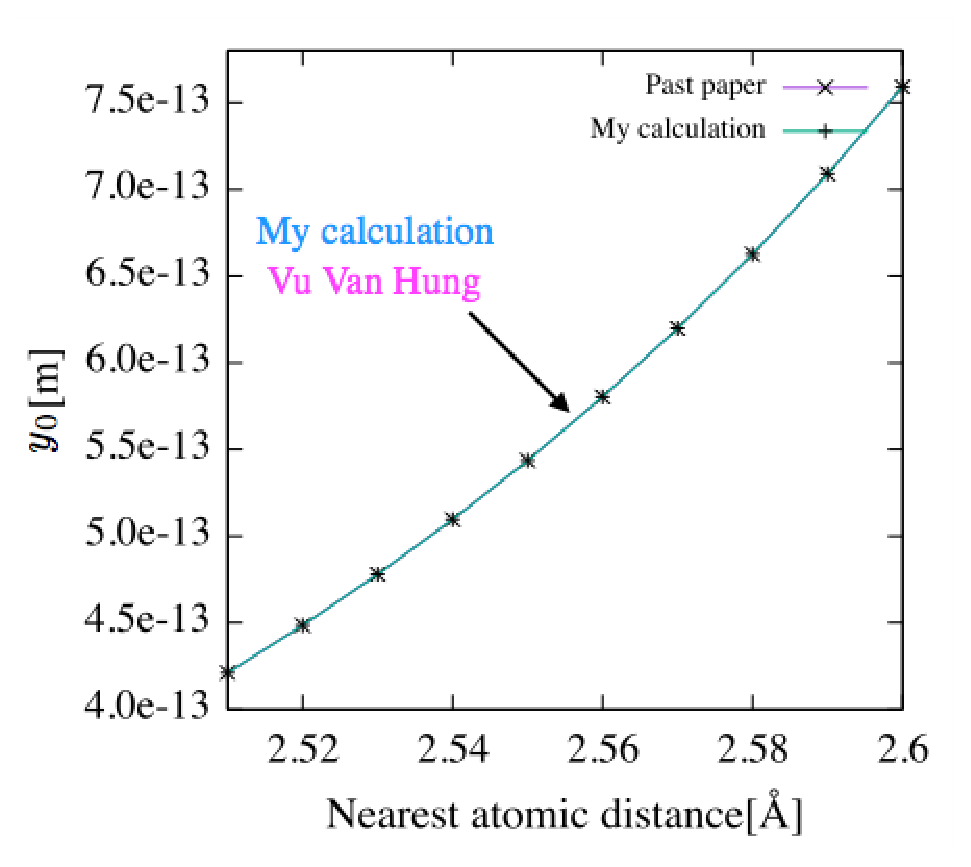
\includegraphics[keepaspectratio, scale=0.42]
  {../image/a4_1_label.eps}
  \subcaption{$T$=100K}\label{a41}
 \end{minipage}
 \begin{minipage}[b]{0.5\linewidth}
  \centering
  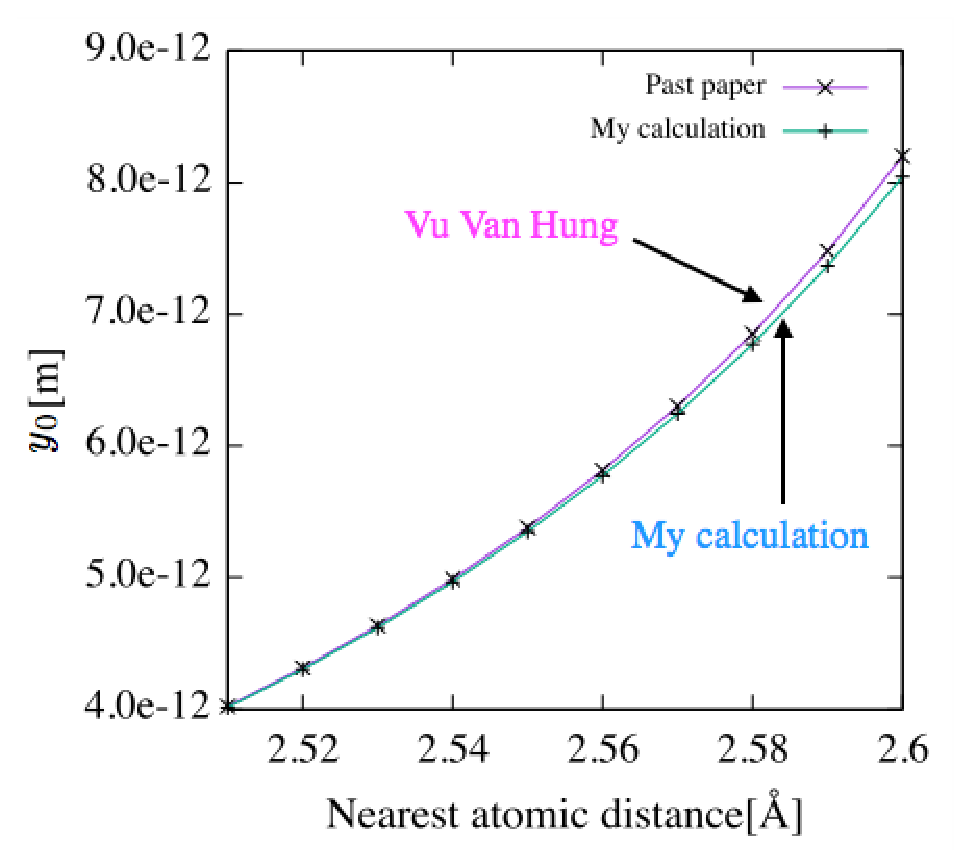
\includegraphics[keepaspectratio, scale=0.42]
  {../image/a4_2_label.eps}
  \subcaption{$T$=900K}\label{a42}
 \end{minipage}
 \caption{導出した$a_4$と参考文献の$a_4$による$y_0$の比較.}\label{fig:vuvana4}
\end{figure}
\section{熱膨張の計算}
\label{sec:heatexpantion} 
前節で外力が無い場合の変位$y_0$の導出をおこなった.本節ではそれを利用した熱膨張の計算について記述する.
まずは$y_0$の導出の際に使用した式(\ref{eq:moment10})に注目する.
左辺$y$は計算者の設定する平衡原子間距離からの変位である.
右辺第一項$y_0$は外力がない場合の変位であり,右辺の残りの項は外力による変位を表している.
ここで$y=y_0$となる場合,右辺第2, 3項が0となる.すなわち,外力による変位が0であり,その時の$y$は外力の影響の無い,熱膨張のみを考慮した変位となる.
$y$と$y_0$の関係を図\ref{fig:yy0}に示す.$y$と平衡原子間距離を足し合わせた原子間距離から,ポテンシャルの2次微分成分$k$,4次微分成分$\gamma$の値がわかる.その後,$k$,$\gamma$の値から$y_0$が算出される.

\begin{figure}[htbp]
 \begin{center}
  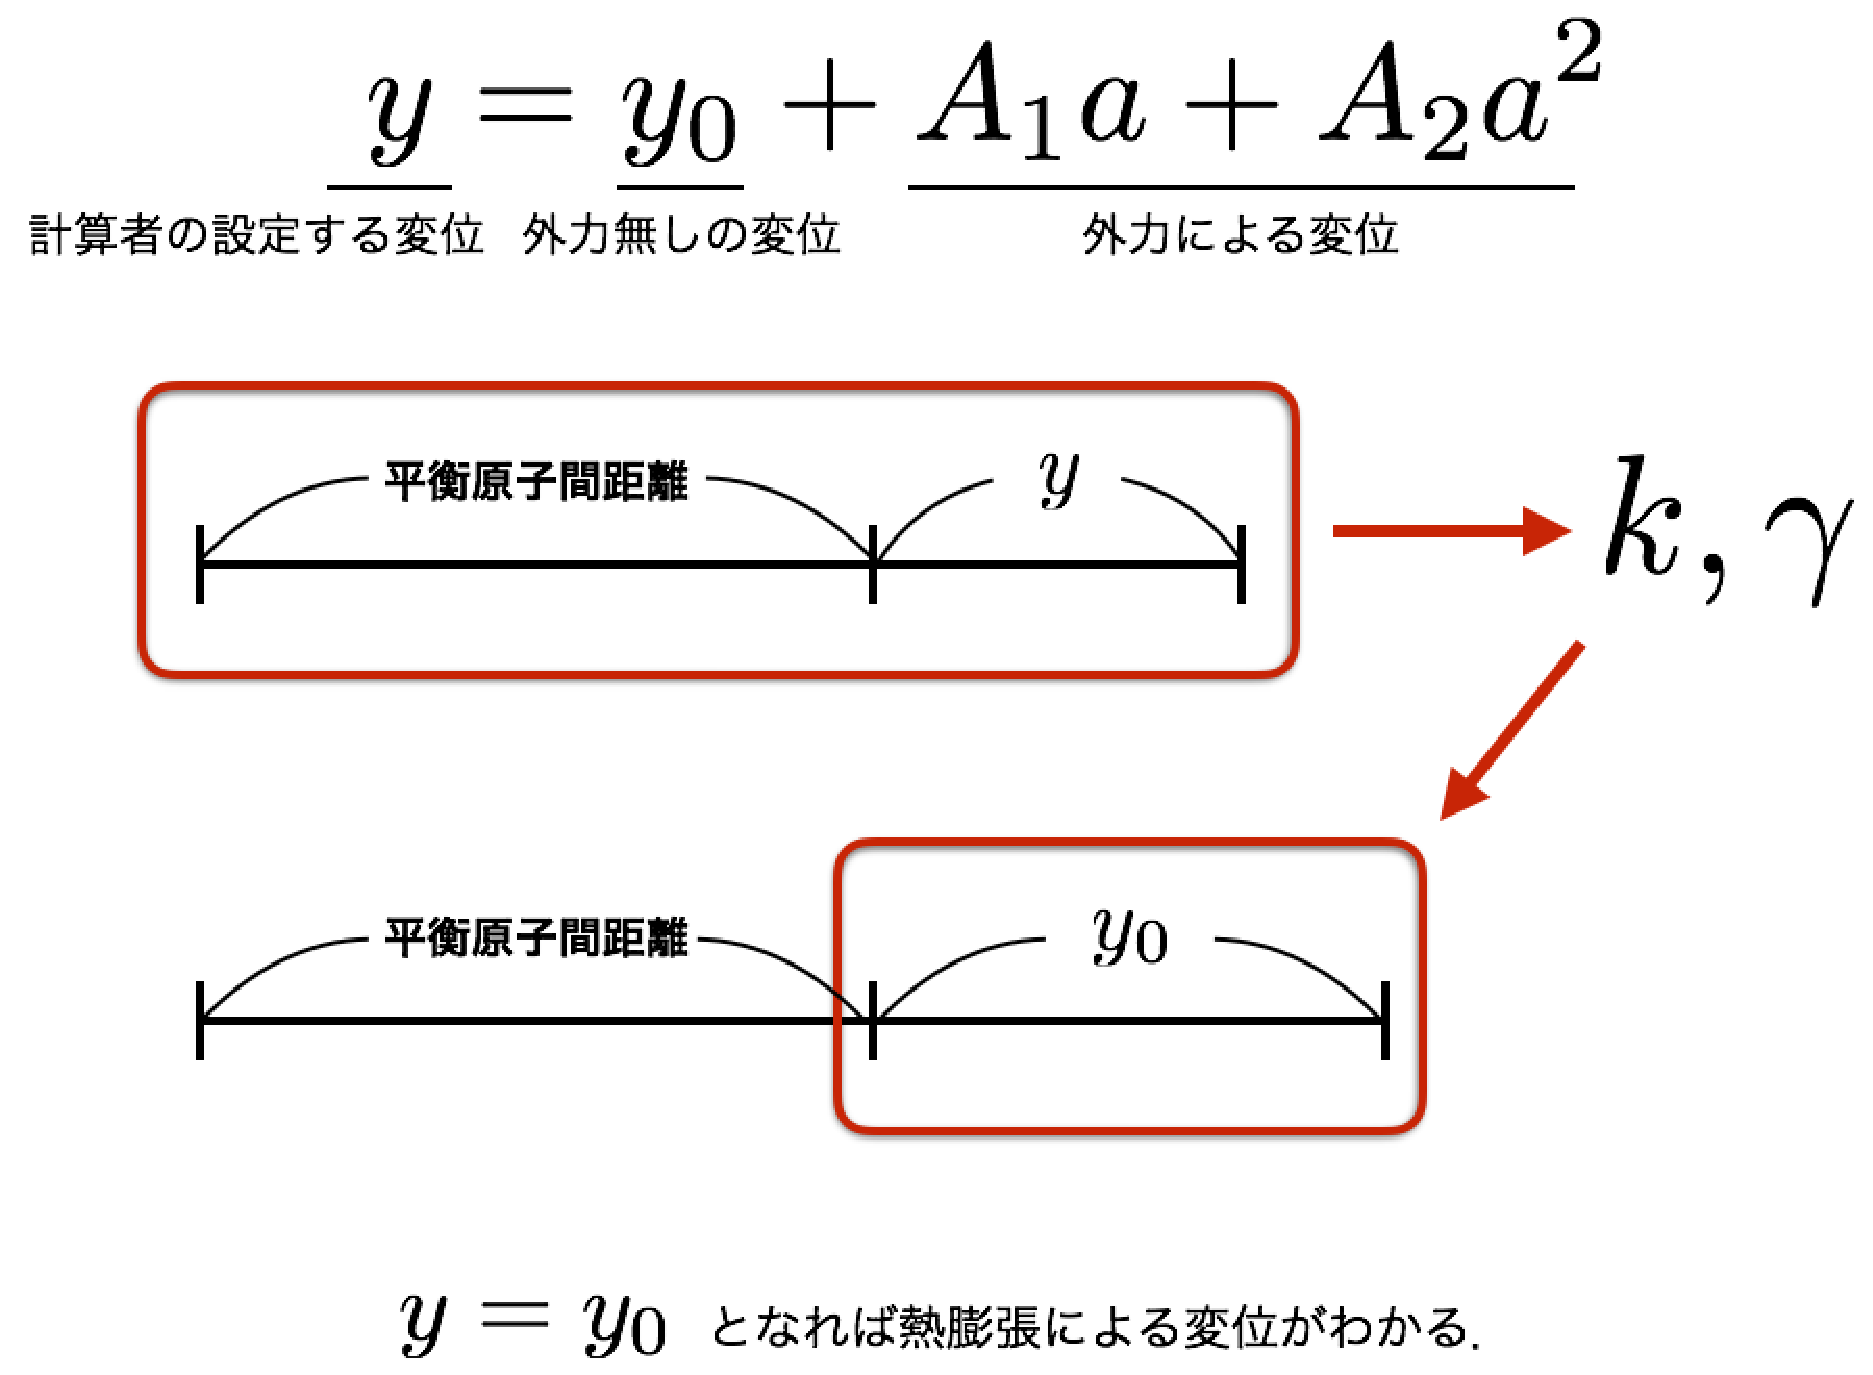
\includegraphics[width=130mm]{../image/fig1.eps}
 \end{center}
 \caption{$y$と$y_0$の関係図.}
 \label{fig:yy0}
\end{figure}


\section{線形結合の自由エネルギー計算}
熱膨張が求まった際,系は外力がない状態である.
その状態のでの原子の変位から$k$, $\gamma$の値を取り出し,自由エネルギーを算出することができる.
Vu Van Hungらによれば,線形結合の自由エネルギー$\psi$は次式となる\cite[p.515]{jindo2}.

\begin{eqnarray}
\label{eq:moment16}
\psi \approx U_0+\psi_0-\frac{N\gamma\theta^2}{6k^2}\left(1+\frac{x \coth x}{2}\right)
-\frac{N\gamma^2\theta^3}{4k^4}\left(1+\frac{x \coth x}{2}\right)(x \coth x + 1)
\end{eqnarray}
\begin{eqnarray}
\label{eq:moment17}
U_0\equiv N\sum_i\varphi_{i0}(|a_i|)
\end{eqnarray}
\begin{eqnarray}
\label{eq:moment18}
\varphi_0 = N\theta[x+\log{(1-e^{-2x})}]
\end{eqnarray}
$U_0$は原子間相互作用によるポテンシャルエネルギーであり,内部エネルギーとも呼ぶ.$\psi_0$は調和振動による自由エネルギーである.式(\ref{eq:moment16})の第3項からは非調和振動による自由エネルギーである.
また$N$は原子数であり,単純に$\psi$全体を$N$倍している.
\section{fcc構造での計算}
\label{sec:fcc}
ここまでは線形結合での計算を示した.実際の格子構造で計算するためには,経験的ペアポテンシャルで格子構造を再現し計算を行わなければならない.本節ではペアポテンシャルを利用したfcc構造での計算手法について記述する.

\subsection{$k$, $\gamma$の導出}
Moment法はポテンシャルの2次微分である$k$,4次微分を6で割った$\gamma$に依存する.
fcc構造では原子配置を考慮すると,式(\ref{eq:moment8})の$k$, $\gamma$の値が次式に置き換わる.
\begin{eqnarray}
\label{eq:moment19}
k \equiv 
\sum_i\left( \frac{\delta^2\varphi_{i0}}{\delta u_{iX}^2}\right),\,
\gamma\equiv\frac{1}{6}\sum_i\left[\left( \frac{\delta^4\varphi_{i0}}{\delta u_{iX}^4} \right)
+6\left( \frac{\delta^4\varphi_{i0}}{\delta u_{iX}^2\delta u_{iY}^2} \right)
\right]
\end{eqnarray}
ここで$X$,$Y$はそれぞれ原子間距離の$x$,$y$成分を表しており,$\frac{\delta^2\varphi_{i0}}{\delta u_{iX}^2}$,$\frac{\delta^4\varphi_{i0}}{\delta u_{iX}^4}$はそれぞれポテンシャルの$x$成分の2次,4次微分を表している.
また,$\frac{\delta^4\varphi_{i0}}{\delta u_{iX}^2\delta u_{iY}^2}$は,ポテンシャルの$x$成分で2次微分,$y$成分で2次微分を表している.
以下に$k$の導出方法を示す.

原子間距離$r$を$x$,$y$,$z$成分で表すと,
\begin{eqnarray}
\label{eq:moment20}
r=\sqrt{x^2+y^2+z^2}
\end{eqnarray}
である.これを考慮してポテンシャル$\varphi(r)$を$x$で2次微分すると次式が得られる.
\begin{eqnarray}
\label{eq:moment21}
\frac{\delta^2\varphi(r)}{\delta x^2}=
\frac{\delta^2 \varphi(r)}{\delta r^2} \frac{x^2}{x^2+y^2+z^2}
-\frac{\delta \varphi(r)}{\delta r} \frac{x^2}{(x^2+y^2+z^2)^{3/2}}
+\frac{\delta \varphi(r)}{\delta r} \frac{1}{\sqrt{x^2+y^2+z^2}}
\end{eqnarray}
これで$\frac{\delta^2\varphi_{i0}}{\delta u_{iX}^2}$の導出は完了であり,ここからは$\sum_i$の計算を行う.
この式にfcc構造の第1近接原子12個,第2近接原子6個の相対的な座標をそれぞれ代入し和を取るとfcc構造の$k$を得ることができる.
\begin{eqnarray}
\label{eq:momentk}
k=
4\frac{\delta^2 \varphi(a_1)}{\delta r^2}
+\frac{8}{a_1}\frac{\delta \varphi(a_1)}{\delta r}
+2\frac{\delta^2 \varphi(a_2)}{\delta r^2}
+\frac{4}{a_2}\frac{\delta \varphi(a_2)}{\delta r}
\end{eqnarray}
ここで,$a_1$は第1近接原子,$a_2$は第2近接原子である.同様の操作で$\sum_i\left(\frac{\delta^4\varphi_{i0}}{\delta u_{iX}^4}\right)$と
$\sum_i\left(\frac{\delta^4\varphi_{i0}}{\delta u_{iX}^2\delta u_{iY}^2}\right)$を計算すると,

\begin{eqnarray}
\label{eq:moment22}
\sum_i \left( \frac{\delta^4\varphi_{i0}}{\delta u_{iX}^4} \right)=
2\frac{\delta^4 \varphi(a_1)}{\delta r^4}
+\frac{12}{a_1}\frac{\delta^3 \varphi(a_1)}{\delta r^3}
-\frac{6}{a_1^2}\frac{\delta^2 \varphi(a_1)}{\delta r^2}
+\frac{6}{a_1^3}\frac{\delta \varphi(a_1)}{\delta r}\nonumber\\
+2\frac{\delta^4 \varphi(a_2)}{\delta r^4}
+\frac{12}{a_2^2}\frac{\delta^2 \varphi(a_2)}{\delta r^2}
-\frac{12}{a_2^3}\frac{\delta \varphi(a_2)}{\delta r}
\end{eqnarray}

\begin{eqnarray}
\label{eq:moment23}
\sum_i \left(\frac{\delta^4\varphi_{i0}}{\delta u_{iX}^2\delta u_{iY}^2}\right)=
\frac{\delta^4 \varphi(a_1)}{\delta r^4}
+\frac{2}{a_1}\frac{\delta^3 \varphi(a_1)}{\delta r^3}
+\frac{3}{a_1^2}\frac{\delta^2 \varphi(a_1)}{\delta r^2}
-\frac{3}{a_1^3}\frac{\delta \varphi(a_1)}{\delta r}\nonumber\\
+\frac{4}{a_2}\frac{\delta^3 \varphi(a_2)}{\delta r^3}
-\frac{6}{a_2^2}\frac{\delta^2 \varphi(a_2)}{\delta r^2}
+\frac{6}{a_2^3}\frac{\delta \varphi(a_2)}{\delta r}
\end{eqnarray}
となり,$\gamma$は
\begin{eqnarray}
\label{eq:gamma}
\gamma=
\frac{4}{3}\frac{\delta^4 \varphi(a_1)}{\delta r^4}
+\frac{4}{a_1}\frac{\delta^3 \varphi(a_1)}{\delta r^3}
+\frac{2}{a_1^2}\frac{\delta^2 \varphi(a_1)}{\delta r^2}
-\frac{2}{a_1^3}\frac{\delta \varphi(a_1)}{\delta r}\nonumber\\
+\frac{1}{3}\frac{\delta^4 \varphi(a_2)}{\delta r^4}
+\frac{4}{a_2}\frac{\delta^3 \varphi(a_2)}{\delta r^3}
-\frac{4}{a_2^2}\frac{\delta^2 \varphi(a_2)}{\delta r^2}
+\frac{4}{a_2^3}\frac{\delta \varphi(a_2)}{\delta r}
\end{eqnarray}
となる.
これによりfcc構造での$k$, $\gamma$がわかった.
\ref{sec:heatexpantion}節で説明した熱膨張の計算は原子が直線上に並ぶ線形結合を前提としている.
そのため,今回導出した$k$, $\gamma$は$x$方向のみに注目して微分を行うことにより,線形結合の熱膨張の計算に対応できるようにしている.
また,$\gamma$には$y$方向の微分も入っているが,これはペアポテンシャルでfcc構造を再現するために混ぜている.


\subsection{自由エネルギーの計算}
ペアポテンシャルによるfcc構造の自由エネルギーの計算は,線形結合の自由エネルギーとは計算式が異なる.
$\gamma_1$,$\gamma_2$を
\begin{eqnarray}
\label{eq:moment24}
\gamma_1=\frac{1}{24}\sum_i \left( \frac{\delta^4\varphi_{i0}}{\delta u_{iX}^4} \right), 
\gamma_2=\frac{1}{4}\sum_i \left(\frac{\delta^4\varphi_{i0}}{\delta u_{iX}^2\delta u_{iY}^2}\right)
\end{eqnarray}
と定義した時,自由エネルギー$\psi$は次式となる\cite[p.516]{jindo2}.
\begin{align}
\label{eq:moment25}
\psi \approx U_0+\psi_0-
3N\left\{ \frac{\theta^2}{k^2}\left[ \gamma_2x^2 \coth^2 x -\frac{2\gamma_1}{3}\left(1+\frac{x \coth x}{2}\right)\right]\right.\nonumber \\
\left. +\frac{2\theta^3}{k^4}\left[\frac{4}{3}\gamma_2^2 x \coth x \left(1+\frac{x \coth x}{2}\right) \right. \right. \nonumber\\
\left. \left. -2(\gamma_1^2+2\gamma_1\gamma_2)\left(1+\frac{x \coth x}{2}\right)(1+x \coth x)\right]\right\}
\end{align}
\begin{eqnarray}
\label{eq:moment27}
\varphi_0 = 3N\theta[x+\log{(1-e^{-2x})}]
\end{eqnarray}
式(\ref{eq:moment16})と同様に$U_0$は原子間相互作用によるポテンシャルエネルギー,$\psi_0$は調和振動による自由エネルギー,	
第3項からは非調和振動による自由エネルギーとなる.$N$は原子数であり,$3N$を全体にかける形になっている.これは$k$,$\gamma$が$x$方向のみをを考慮にいれており,残りの$y$,$z$方向の値を加えるためである.
%moment法
\chapter{計算手法}
本章では,Moment法による計算手法,また,比較対象である,Phonon-DOS法,Phonopyについて記述する.

\section{熱膨張決定のアルゴリズム}
\ref{sec:heatexpantion}節で熱膨張による変位の求め方について述べ,$y$=$y_0$の時の$y$が熱膨張による変位だとわかった.
$y_0$は$k$と$\gamma$を介して$y$に依存する関数であり,$y$の変化に合わせて$y_0$を変化することになる.
$y$=$y_0$となる$y$を決定するアルゴリズムは次のようになる.
\begin{enumerate}
 \item 平衡原子間距離$a_0$を定める.
 \item 計算者が決定する変位$y$に一定の値を足す.
 \item $a_0$+$y$から原子間距離が求まる.
 \item 3.の値から$k$, $\gamma$を求める.
 \item $k$, $\gamma$から$y_0$を求める.
 \item $y$が$y_0$を超えるまで2-5.を繰り返す.
 \item $y$が$y_0$を越えたら,越える前まで戻す.
 \item $y$に足していた一定の値を10で割り2.に戻る.
 \item 2-8.を繰り返すことにより,$y=y_0$の精度を上げる.
\end{enumerate}
このアルゴリズムを図\ref{fig:algo}に示す.
\begin{figure}[htbp]
 \begin{center}
  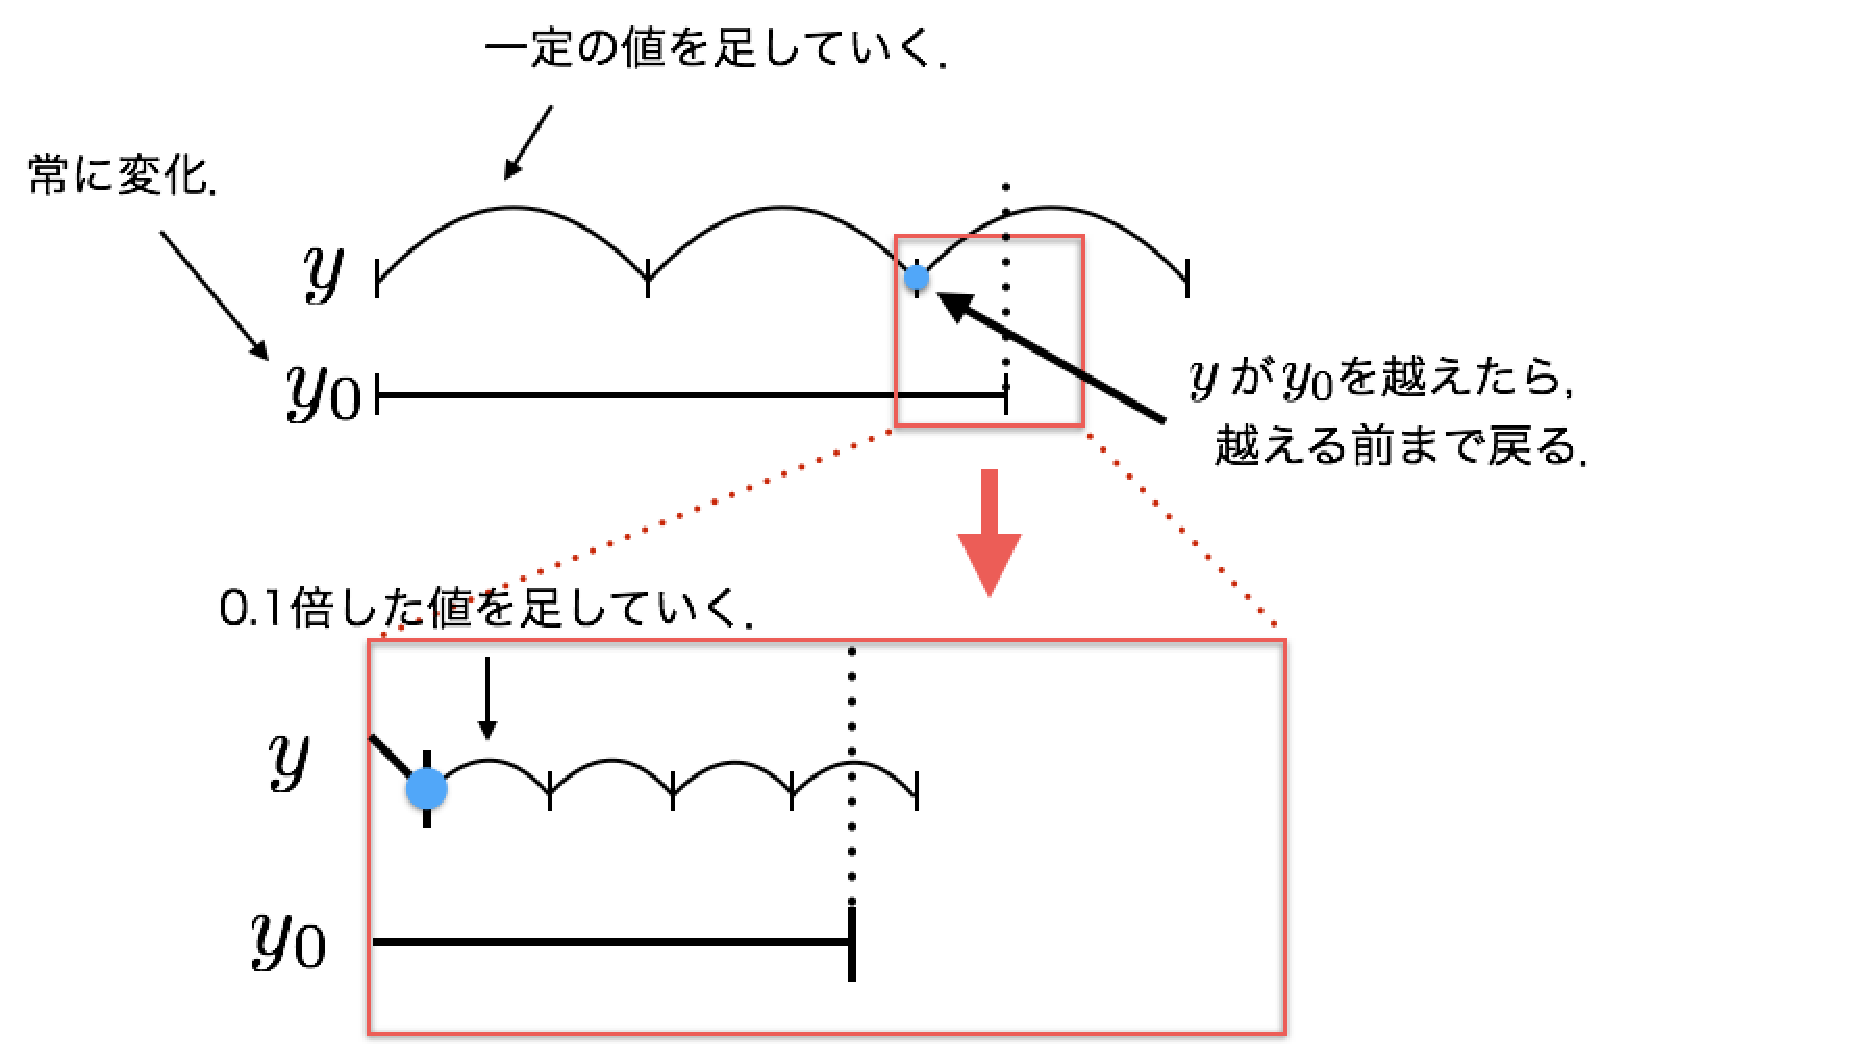
\includegraphics[width=130mm]{../image/fig2.eps}
 \end{center}
 \caption{熱膨張による変位決定アルゴリズム.}
 \label{fig:algo}
\end{figure}

\section{ペアポテンシャルによる計算}
\ref{sec:fcc}節でペアポテンシャルを利用したfcc構造での計算方法について記述した.
今回使用した経験的ペアポテンシャルは次式となる.
\begin{eqnarray}
\label{eq:method1}
U(r)=\frac{D}{n-m}\left[m{\left(\frac{r_0}{r}\right)}^n-n{\left(\frac{r_0}{r}\right)}^m\right]
\end{eqnarray}
このポテンシャルはLennart-Jones型であり,$r$が原子間距離,$r_0$が最安定距離,$D$,$n$,$m$は原子によって定まるパラメータである.また,$a_0$は計算に用いた平衡原子間距離である.
Cu, Ag, Auのパラメータを表\ref{tb:potential}に示す.例としてCuのポテンシャルの概形を図\ref{fig:lj}に示す.
\begin{table}[htbp]
\caption{ポテンシャルのパラメータ.}
  \label{tb:potential}
  \centering
  \begin{tabular}{cccccc}\hline
    元素 & $D$[J] & $n$ & $m$ & $r_0[\mathrm{\AA}$] & [$a_0\mathrm{\AA}$]\\ \hline \hline
    Cu & 2.8480708$\times10^{-20}$ & 9.0 & 5.5 & 2.5487 & 2.512666\\
    Ag & 2.295742359$\times10^{-20}$ & 11.5 & 5.50 & 2.876 & 2.846223\\
    Au & 3.23278851$\times10^{-20}$ & 10.5 & 5.50 & 2.8751 & 2.841578\\ \hline
  \end{tabular}
\end{table}
\begin{figure}[htbp]
 \begin{center}
  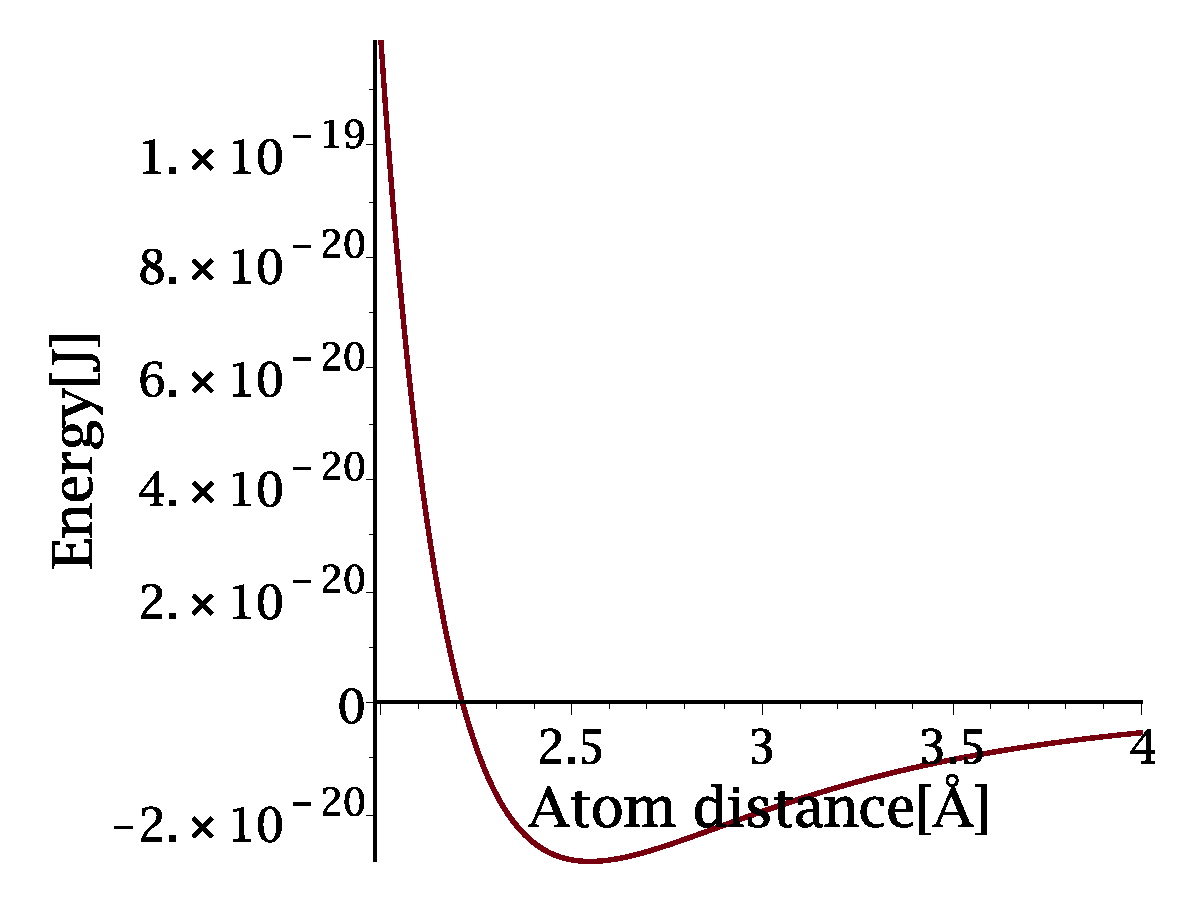
\includegraphics[width=100mm]{../image/lj.eps}
 \end{center}
 \caption{Cuのポテンシャルの概形.}
 \label{fig:lj}
\end{figure}
\section{VASPの導入}
Moment法はペアポテンシャルを前提としているが,VASPでの第一原理計算の結果の導入を試みる.
fcc構造であるCu, Ag, Au, Alのユニットセルの格子を変化させ,それぞれの基底状態のエネルギーを求める.
そして,フィッティングを行い最近接原子間距離とエネルギーについてのポテンシャル関数を作る.
このポテンシャル関数はVASPによる計算のため$x$,$y$,$z$全方位を考慮したポテンシャルである.
そのため,そのまま2次微分を$k$, 4次微分を6で割ったものを$\gamma$として式(\ref{eq:moment15})の$y_0$に入れて計算をしても$y_0$が線形結合を前提としているため上手く熱膨張を再現できない.
今回はfcc構造が当方的であることから,単純にポテンシャルを3で割り線形結合を表現することにする.
自由エネルギーの計算には式(\ref{eq:moment16})の線形結合の自由エネルギーに$k$, $\gamma$を代入し,式(\ref{eq:moment27})と同様に,$x, y, z$方向を考慮して3倍した値を自由エネルギーとする.
\subsection{VASP(Vienna Ab-initio Simulation Package)}
VASP は,密度汎関数法による平面波・擬ポテンシャル法を用いた第一原理計算プログラムパッケージで
ある.本研究ではこのソフトを用いて第一原理計算をおこなった.擬ポテンシャル法は原子の内殻電子を
除いた価電子だけを考慮する方法である.そのため,全電子を計算するフルポテンシャル法に比べ比較的
高速な計算が可能となる.また,内殻電子は化学結合や物性に影響を与えることが少ないのため,擬ポテ
ンシャル法であっても十分な精度で計算ができる.本研究の計算にはPAW法(Projector Augmented Wave method)を使用した.PAW法は擬ポテンシャル法を採用しながらも,内殻付近の挙動を比較的精度よく再現することができる計算手法である.VASPの計算条件は入力ファイルであるINCAR, KPOINTSにより決定される.本研究の中で比較をおこなった計算条件を以下に記す.
\begin{description}
 \item[ENCUT]\mbox{}\\ 
	    Cut-off energyと呼ばれる値である.
	    これは,どれだけ短波長の平面波を使い,波動関数をより精密に表現するかを決めるパラメータである.
	    入力した値が大きいほど,短波長の平面波を考慮に入れた計算を行うことができる.
 \item[KPOINTS]\mbox{}\\
	    波動関数を$k$空間で展開する際にどれだけの点をとるか決定することができる.
	    計算の精度に直接関わるパラメータである.
\end{description}


\subsection{フィッティング}
fcc構造のユニットセルに対して,VASPの構造最適化によって得られた格子定数を0.95倍から1.10倍まで0.01刻みで変化させエネルギーの計算を行い,得られた16点に対してフィッティングをおこなった.図\ref{fig:examplefit}にCuのフィッティングを示す.
\begin{figure}[htbp]
 \begin{center}
  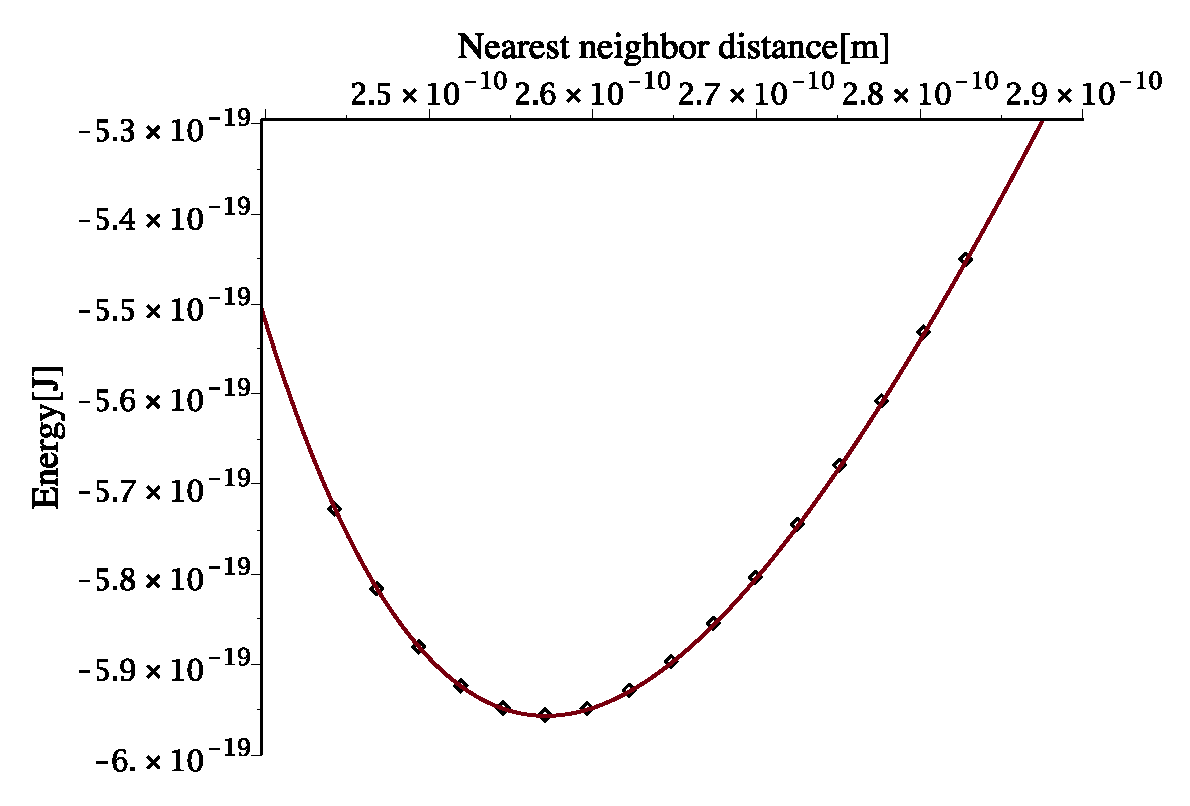
\includegraphics[width=100mm]{../image/fit5.eps}
 \end{center}
 \caption{Cuのフィッティング.}
 \label{fig:examplefit}
\end{figure}
今回フィッティングに使用した関数の$n$次数までの基本形は次式となる.
\begin{eqnarray}
\label{eq:method2}
U(r)=a_0+a_1(r-x_0)+a_2(r-x_0)^2+\cdots+a_n(r-x_0)^n
\end{eqnarray}
ここで,$x_0$はポテンシャルの最安定距離であり,関数全体を$x$方向に$x_0$だけずらしフィッティング精度を高めている.
フィッティングして得られたポテンシャルの2次,4次微分を利用することとなるが,4次微分となるとフィッティングの精度の影響を大きく受けてしまう.
また,フィッティング関数の次数もどこまで取れば最適なのか検討する必要がある.
図\ref{fig:fit}にフィッティングで得られた関数の4次微分の結果を示す.

\begin{figure}[htbp]
 \begin{minipage}[b]{0.5\linewidth}
  \centering
  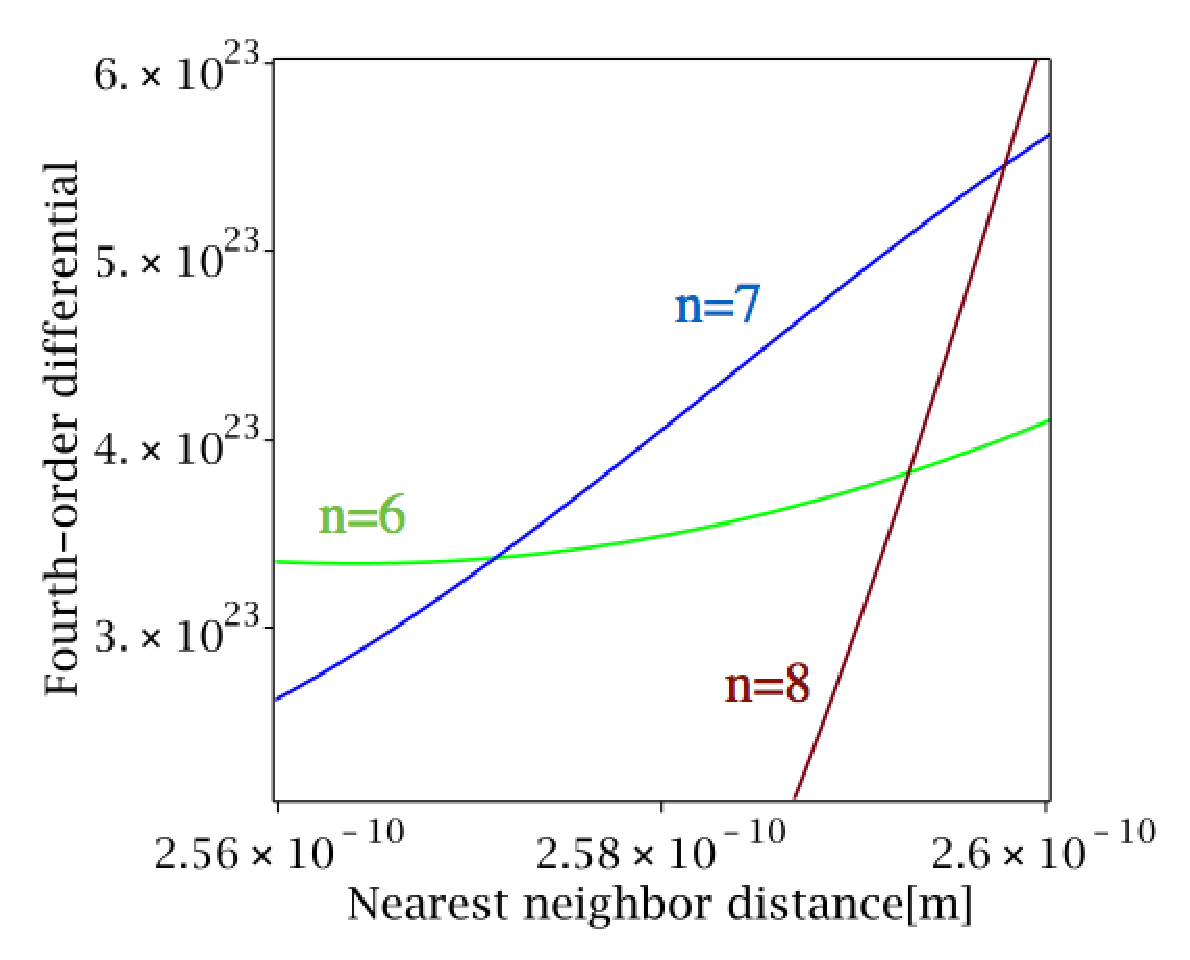
\includegraphics[keepaspectratio, scale=0.41]
  {../image/fit1label.eps}
  \subcaption{Cu, ENCUT=500, KPOINTS=6$\times$6$\times$6.}\label{fit1}
 \end{minipage}
 \begin{minipage}[b]{0.5\linewidth}
  \centering
  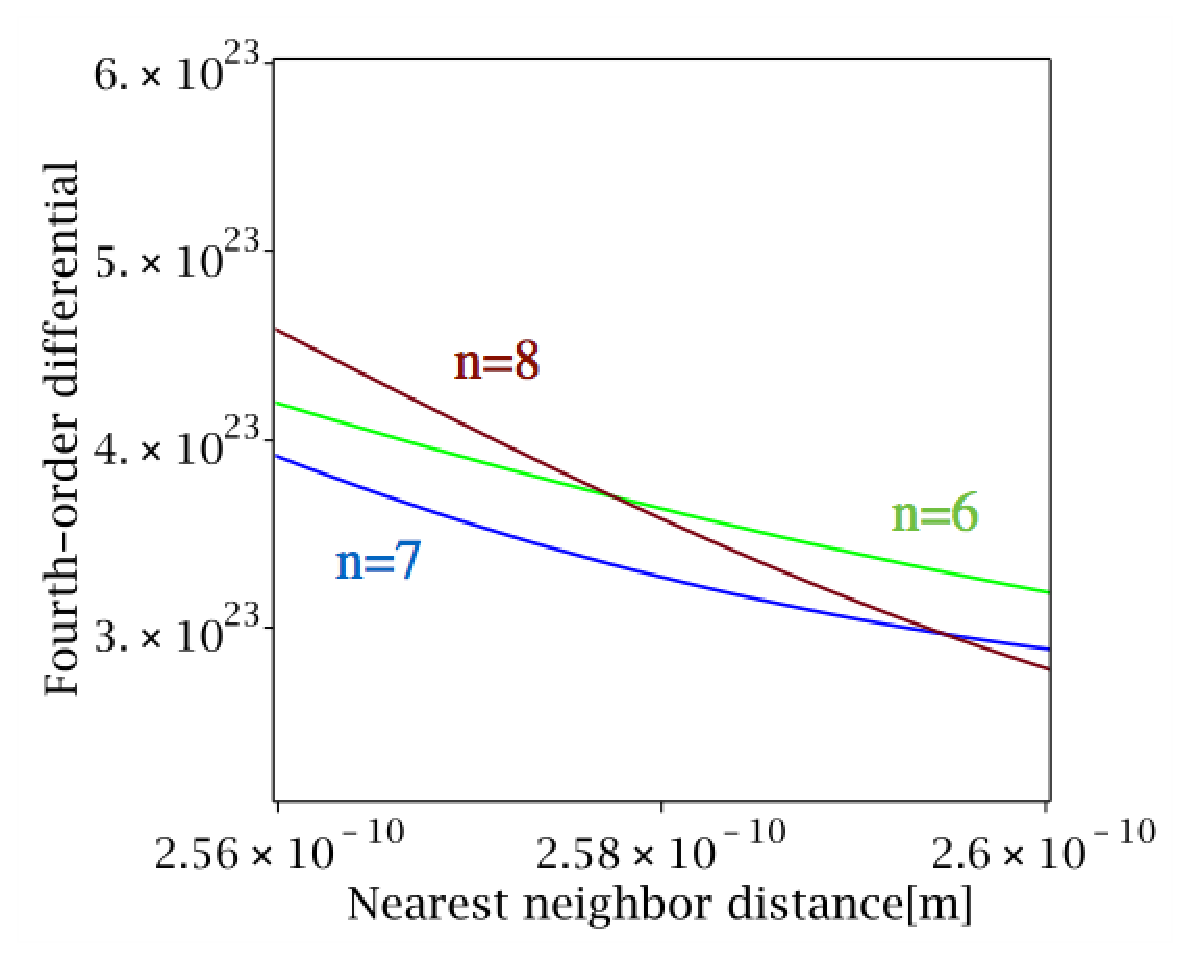
\includegraphics[keepaspectratio, scale=0.41]
  {../image/fit2label.eps}
  \subcaption{Cu, ENCUT=750, KPOINTS=12$\times$12$\times$12.}\label{fit2}
 \end{minipage}
 %\hspace{10cm}
 \begin{minipage}[b]{0.5\linewidth}
  \centering
  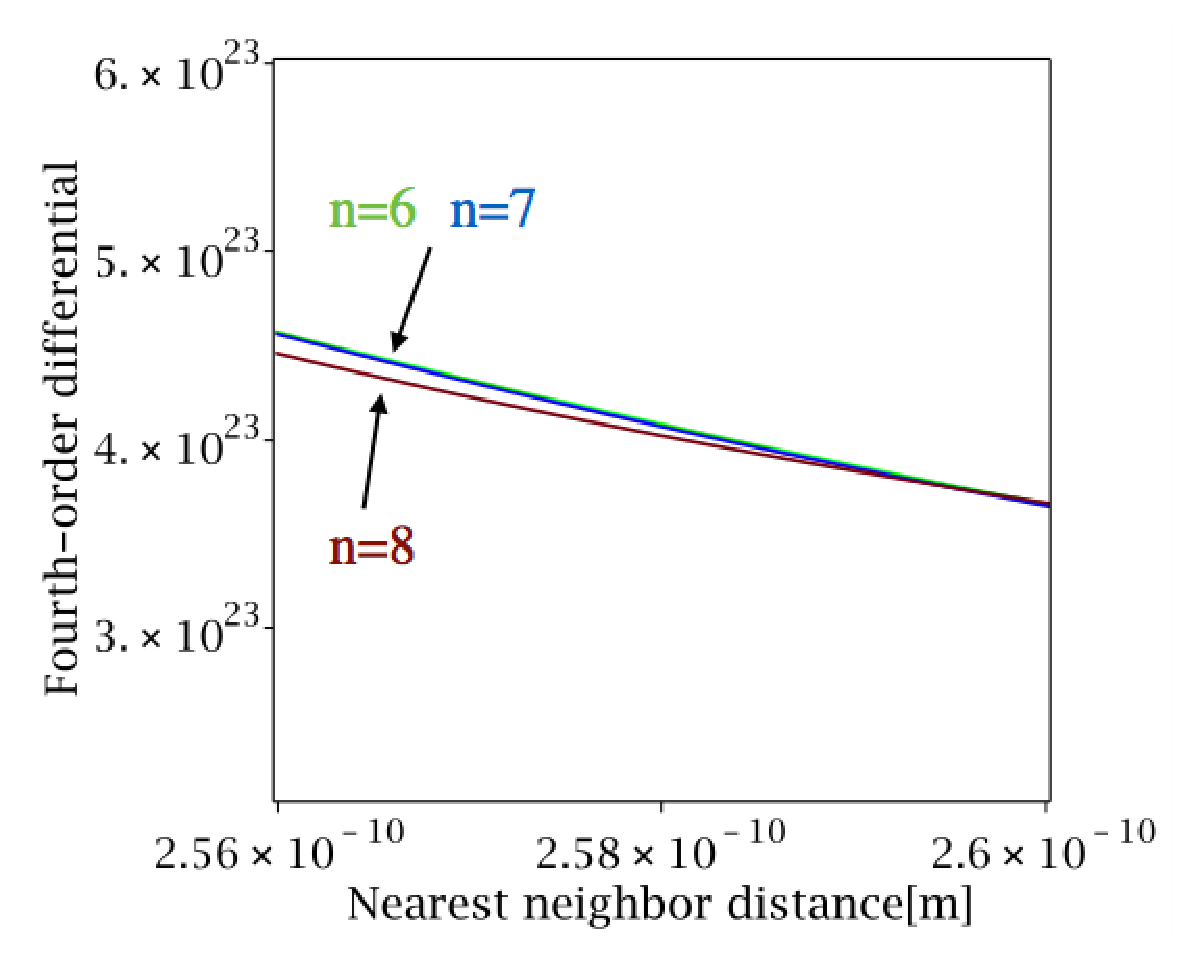
\includegraphics[keepaspectratio, scale=0.41]
  {../image/fit3label.eps}
  \subcaption{Cu, ENCUT=1000, KPOINTS=36$\times$36$\times$36.}\label{fit3}
 \end{minipage}
 \begin{minipage}[b]{0.5\linewidth}
  \centering
  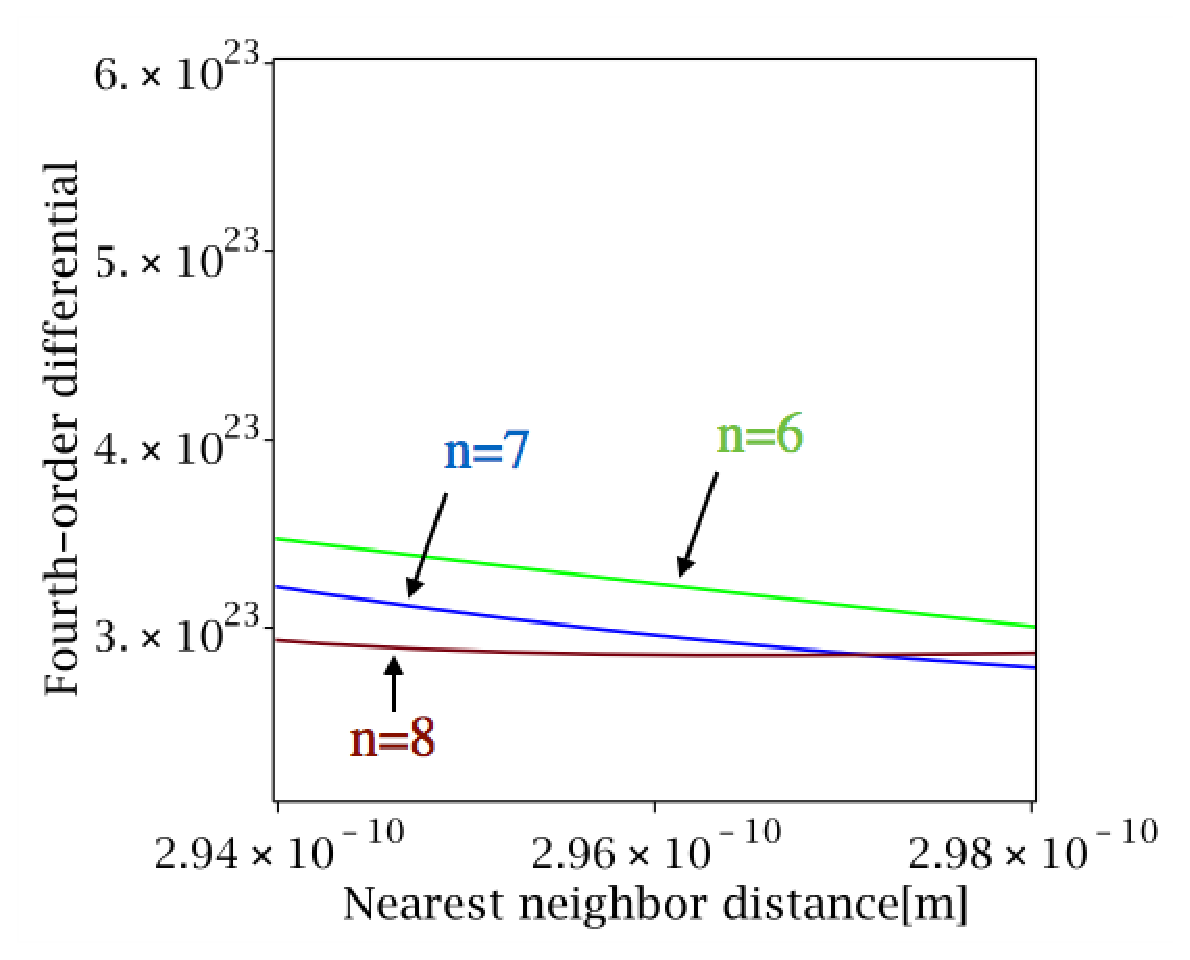
\includegraphics[keepaspectratio, scale=0.41]
  {../image/fit_ag_label.eps}
  \subcaption{Ag, ENCUT=1000, KPOINTS=36$\times$36$\times$36.}\label{fit4}
 \end{minipage}
  \begin{minipage}[b]{0.5\linewidth}
  \centering
  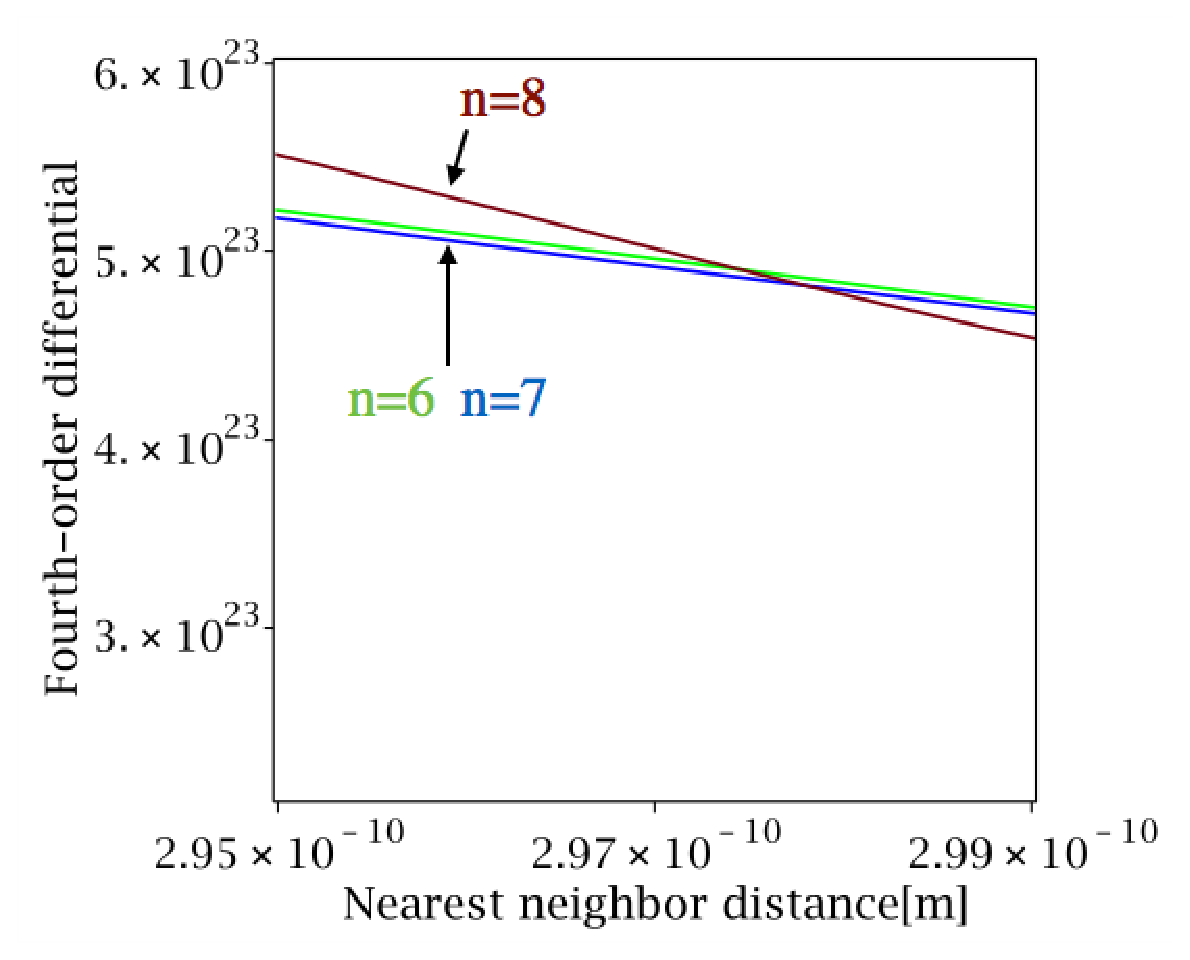
\includegraphics[keepaspectratio, scale=0.41]
  {../image/fit_au_label.eps}
  \subcaption{Au, ENCUT=1000, KPOINTS=36$\times$36$\times$36.}\label{fit5}
 \end{minipage}
 \begin{minipage}[b]{0.5\linewidth}
  \centering
  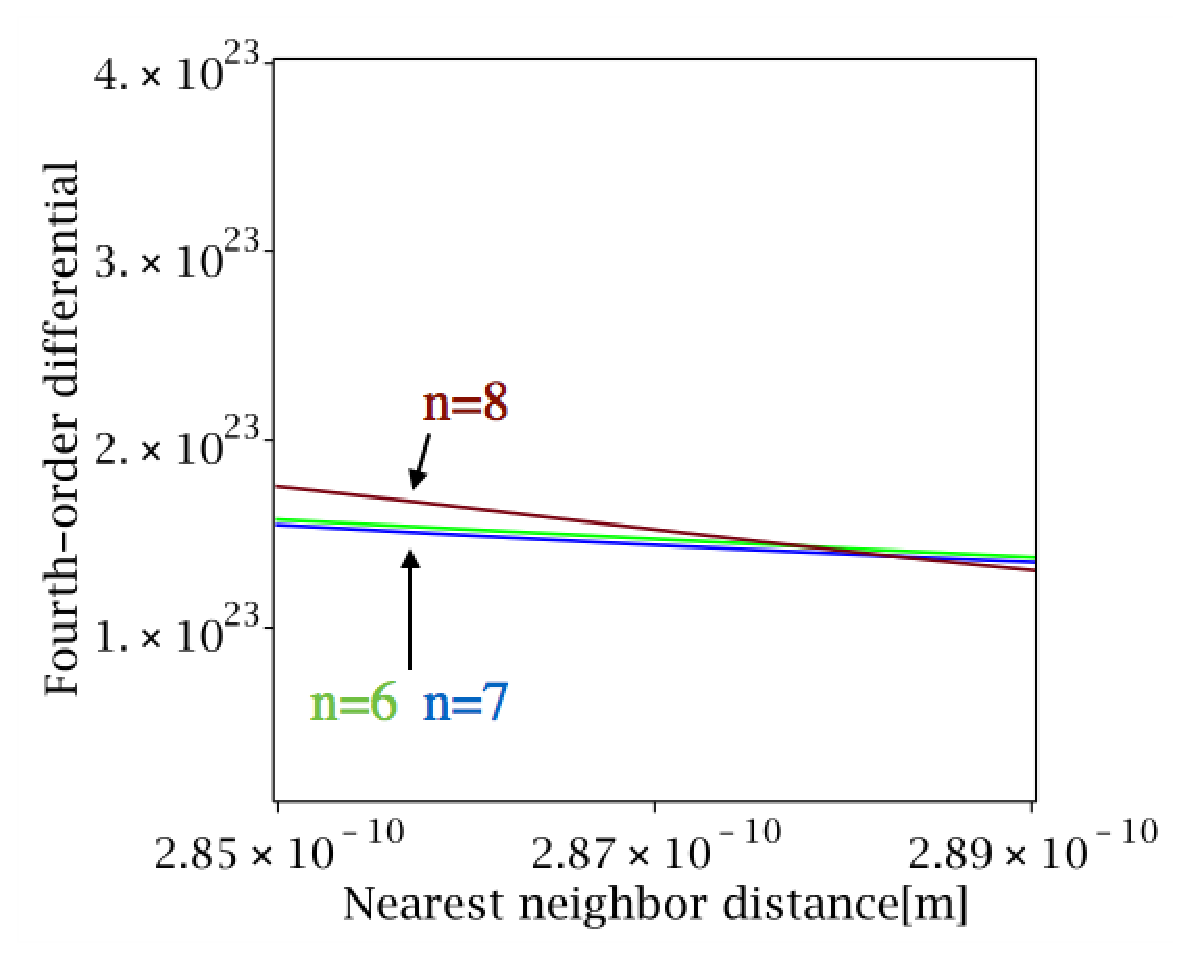
\includegraphics[keepaspectratio, scale=0.41]
  {../image/fit_al_label.eps}
  \subcaption{Al, ENCUT=1000, KPOINTS=36$\times$36$\times$36.}\label{fit6}
 \end{minipage}
 \caption{計算精度とフィッティング関数の次数によるポテンシャルの4次微分の値.$n$はフィッティングに使用した関数の次数である.ENCUT, KPOINTSはVASPの計算精度に関わるパラメータである.}\label{fig:fit}
\end{figure}

これは,フィッティング関数の次数とVASPの計算精度に関わるパラメータENCUTとKPOINTSによって,4次微分がどのような値をとるか示している.
横軸には各元素のVASPの構造最適化によって得られた最安定距離周辺を取っている.
図\ref{fig:fit}(\subref{fit1}),(\subref{fit2}),(\subref{fit3})はVASPの計算精度を変えることによって,Cuのフィッティング関数の4次微分にどのように変化するか示している.計算精度を高めることによって値が収束していることがわかる.
また,(\subref{fit4}),(\subref{fit5}),(\subref{fit6})は(\subref{fit3})と同じ計算条件のAg, Au, Alの結果である.
それぞれの結果を見るとAgを除けば6次と7次のフィッティング関数の値がほぼ一致するという結果であった.
8次のフィッティング関数に7次まででは拾えていない成分がある可能性もあるが,今回は4次微分した際に3次の項まで残れば十分であると判断し7次のフィッティング関数を用いてフィッティングを行う.
また,VASPでの計算条件はENCUT=1000,KPOINTS=36$\times$36$\times$36とする.
VASPの構造最適化で得られた実際の計算に用いた平衡原子間距離$a_0$を表\ref{tb:a0all}に示す.
7次のフィッティングで得られた2次微分,4次微分の値を図\ref{fig:allkgamma}に示す.
この図は,各元素の2次微分と4次微分のそれぞれ平衡原子間距離$a_0$からプロットし,値や傾きの比較が行えるようになっている.
\begin{table}[htbp]
\caption{VASPの構造最適化によって得られた平衡原子間距離$a_0$.}
  \label{tb:a0all}
  \centering
  \begin{tabular}{ccccc}\hline
    元素 & Cu & Ag & Au & Al\\ \hline \hline
    $a_0[\mathrm{\AA}]$ & 2.571623 & 2.944229 & 2.951082 & 2.856525\\ \hline
  \end{tabular}
\end{table}

\begin{figure}[htbp]
 \begin{minipage}[b]{0.5\linewidth}
  \centering
  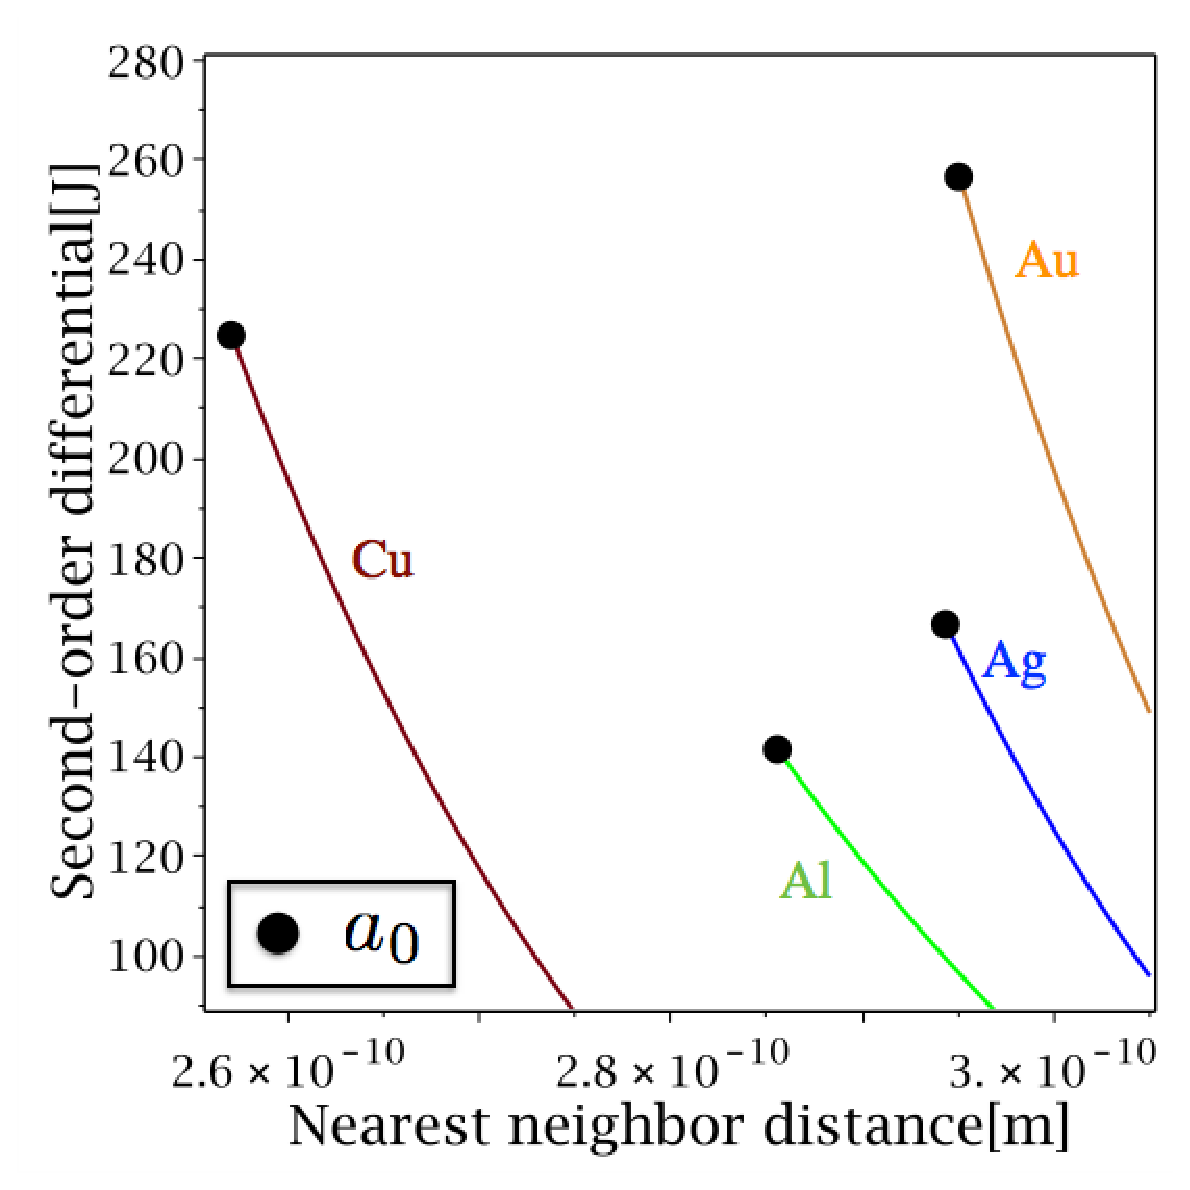
\includegraphics[keepaspectratio, scale=0.41]
  {../image/all_k_label.eps}
  \subcaption{フィッティングした関数の2次微分.}\label{allk}
 \end{minipage}
 \begin{minipage}[b]{0.5\linewidth}
  \centering
  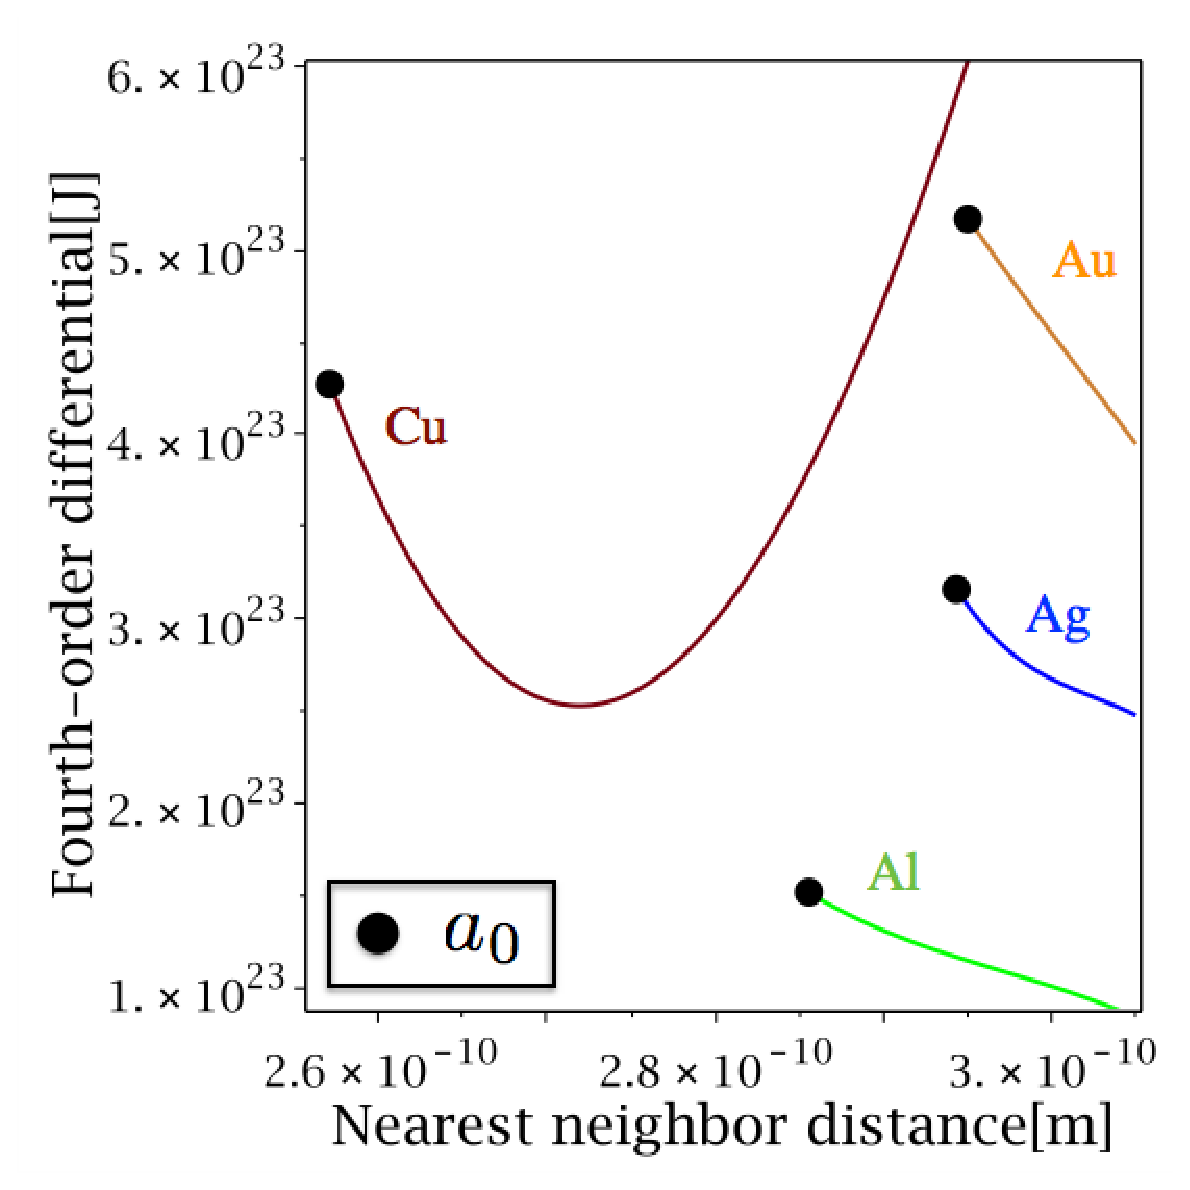
\includegraphics[keepaspectratio, scale=0.41]
  {../image/all_gamma_label.eps}
  \subcaption{フィッティングした関数の4次微分.}\label{allgamma}
 \end{minipage}
  \caption{各元素のフィッティングによって得られた関数の2次微分,4次微分の分布.}\label{fig:allkgamma}
\end{figure}


\section{MedeA}
データベースと第一原理計算を統合した材料設計支援のためのソフトウェアであり, 
構造の検索, 構築, 編集, 計算, 解析までを1つのプラットフォームで行うことができる商用ソフトである.
MedeAには格子振動に関連する物性を計算するためのツールとしてMedeA-Phononが搭載されており,擬調和振動子近似に基づき基底状態におけるPhonon分散曲線からPhonon状態密度を計算することができ,Phonon-DOS法を用いて自由エネルギーを算出することができる.
本研究ではMoment法の比較対象として,Cu,Ag,Au,Alの熱膨張と自由エネルギーの計算をおこなった.
Phonon-DOS法は熱振動効果を考慮しているが熱膨張は取り入れることができず,一定体積における自由エネルギーの計算を行うことになる.
そのため熱膨張を見積もるためには計算モデルの格子定数を変化させ,それぞれの自由エネルギーを算出し各温度における最安定構造を見つけ出す必要がある.
\subsection{Phonon-DOS法}
有限温度の効果を取り込んだ自由エネルギーは基底状態における系のトータルエネルギーと振動自由エネルギーの総和で表せられ次式で求めることができる\cite{kittel}.
\begin{eqnarray}
\label{eq:phonon}
F(a,T)=E(a)+k_BT\int_0^\infty n(\omega)\left[
2\sinh\left(\frac{\hbar\omega}{2k_BT}\right)
\right]d\omega
\end{eqnarray}
$E(a)$は基底状態の系のエネルギー,$k_B$はボルツマン定数,$T$は温度,$\omega$はPhonon分散曲線における振動数,$n(\omega)$はPhonon状態密度(Phonon-DOS),$\hbar$はプランク定数を$2\pi$で割った値である.
右辺第一項は基底状態におけるトータルエネルギー,右辺第二項は振動自由エネルギーを表している.
この式から振動自由エネルギーはPhonon状態密度から見積もることができ,Phonon状態密度を現実の系に近づけることが計算精度を高めることに繋がる.

\section{Phonopy}
東後篤史が制作したオープンソースのソフトウェアでありPhonon状態密度や分散曲線,自由エネルギーな
どの様々な有限温度の物性を第一原理計算ソフトと連携することで計算することができる\cite{phonopy}.
Phonopyという名前の由来は,Phonon計算をプラグラミング言語Pythonで行うことから来ている.
CLI(Command Line Interface)であり,Pythonのパッケージ管理システムであるpipとcondaに対応しており,環境構築も容易に行うことができる.
Phonon計算の簡単な流れは次のようになる.
\begin{enumerate}
 \item Phonopyにより原子を微小移動させたモデルを作成する.
 \item そのモデルに第一原理計算を行い,結果から力の定数を取り出す.
 \item 力の定数からPhonopyがPhonon計算を行う.
\end{enumerate}

Phonopyは内部エネルギー(基底状態のエネルギー)を考慮に入れた熱膨張を計算することが可能であり,それにより内部エネルギーと熱膨張を考慮に入れた自由エネルギーを見積もることができる.
本研究ではMoment法の比較対象として,Phonopyを用いて,Cu,Ag,Au,Alの熱膨張,自由エネルギー,内部エネルギーと熱膨張を考慮にいれた自由エネルギーの比較をおこなった.
\subsection{計算精度の検討}
PhonopyはVASPの計算から力の定数を取り出しPhononを計算するためVASPの計算結果に大きく依存する.
また,Phonon計算時に生じた誤差は温度の上昇とともに増大するため,高温域の状態を確認したいのであれば計算精度を高める必要がある.
計算精度による熱膨張の変化を図\ref{fig:phonopy}に示す.
図\ref{fig:phonopy}(\subref{phonopy1}),(\subref{phonopy2}),(\subref{phonopy3})はPhonopyによるAlの熱膨張の結果である.VASPの計算精度に関わるパラメータENCUTとKPOINTSを変えることによって,Phonopyの熱膨張の計算結果がどのように変わるか示している.
左側のグラフは横軸に体積,縦軸に自由エネルギーを取っており,各温度でフィッティングを行い最安定の体積を求めている.一番上のフィッティングカーブが0Kであり,一番下が1000Kと100K刻みで計算をしている.
中央のグラフは横軸に温度,縦軸に体積をとっており,左のグラフから得られる各温度での最安定の体積である..
右側のグラフは横軸に温度,縦軸に体積膨張係数を取っており,中央のグラフの温度微分である.
(\subref{phonopy1}),(\subref{phonopy2}),(\subref{phonopy3})を比較すると左側のグラフの高温域の点のずれが計算精度を高めることによって小さくなることがわかる.
このずれがフィッティングによる最安定点の決定に与える影響は大きく,体積膨張係数を見ればその影響力の大きさがよくわかる.
(\subref{phonopy3})の結果も,よく見ると点が線の中心からずれているため本来であればもっと計算精度を高めたいところである.
しかし,計算時間の都合もあり本研究のPhonopyの計算条件にはENCUT750,KPOINTS=12$\times$12$\times$12を使用した.


\begin{figure}[htbp]
 \begin{minipage}[b]{1.0\linewidth}
  \centering
  \includegraphics[keepaspectratio, scale=0.45]
  {../image/figure_1.png}
  \subcaption{ENCUT=500, KPOINTS=6$\times$6$\times$6.}\label{phonopy1}
 \end{minipage}
  \begin{minipage}[b]{1.0\linewidth}
  \centering
  \includegraphics[keepaspectratio, scale=0.45]
  {../image/figure_2.png}
  \subcaption{ENCUT=500, KPOINTS=12$\times$12$\times$12.}\label{phonopy2}
 \end{minipage}
   \begin{minipage}[b]{1.0\linewidth}
  \centering
  \includegraphics[keepaspectratio, scale=0.45]
  {../image/figure_3.png}
  \subcaption{ENCUT=750, KPOINTS=12$\times$12$\times$12.}\label{phonopy3}
 \end{minipage}
 \caption{VASPの計算精度によるPhonopyのAlの熱膨張の計算誤差.}\label{fig:phonopy}
\end{figure}



%計算手法
\chapter{計算結果}
VASPを導入したMoment法,Lennerd-Jones型経験的ペアポテンシャルを用いた従来のMoment法,MedeA, Phonopyによる結果の比較を行う.図内のラベルには結果をそれぞれ,MomentVASP, MomentLJ, MedeA, Phonopyと表記しており,今後はこの名称で扱うことにする.
\section{熱膨張}
熱膨張による最近接原子間距離の温度依存を図\ref{fig:heatexpantion}に示す.この結果から得られる線膨張係数を図\ref{fig:heatexpantion2}に実験値とともに示す.
MomentLJの0Kの最近節原子間距離が他の結果と大きな差があるのは使用したペアポテンシャルの最安定距離がVASPによる基底状態の最安定距離とずれているためである.また,高温域で現実的ではない加速的な熱膨張をしており$k$,$\gamma$が負の値を取り計算不可となり結果が途切れている.MomentLJとMomentVASPを比較すると,後者がMedeA, Phonopy, 実験値に近い結果を出していることがわかる.
MomentLJ,MomentVASPともに100K以下の低温域で現実的ではない熱膨張を示しており\ref{sec:he_100k}節で原因の検証を行う.
MomentVASPのCu, Ag, Auに着目するとAgの高温域での加速的な熱膨張を除いてPhonopy, MedeAに劣らず実験値に近い結果が出ている.
Phonopy, MedeAのAuの結果が大きく熱膨張しているのは,格子を大きく伸ばしたAuにおいてPhonon状態密度に負の値が多く混ざり自由エネルギーが正確に算出できなかったためである.
そのため,AuはPhonon-DOS法では熱膨張を上手く再現できなかったが,Phononとは違うアプローチで計算を行うMomentVASPでは実験値に近い熱膨張係数を得ることができている.
Alに関してはMedeA, Phonopyが上手く実験値を再現できているがMomentVASPでは熱膨張が小さいという結果となった.
これらの結果と図\ref{fig:allkgamma}を比べると$k$, $\gamma$の傾きが変わらなければ直線的な熱膨張になることがわかる.
MomentVASPのAgの高温域における熱膨張は$\gamma$の傾きの変化が他の元素に比べて大きいことが原因だと考えられる.
\begin{figure}[htbp]
 \begin{minipage}[b]{0.5\linewidth}
  \centering
  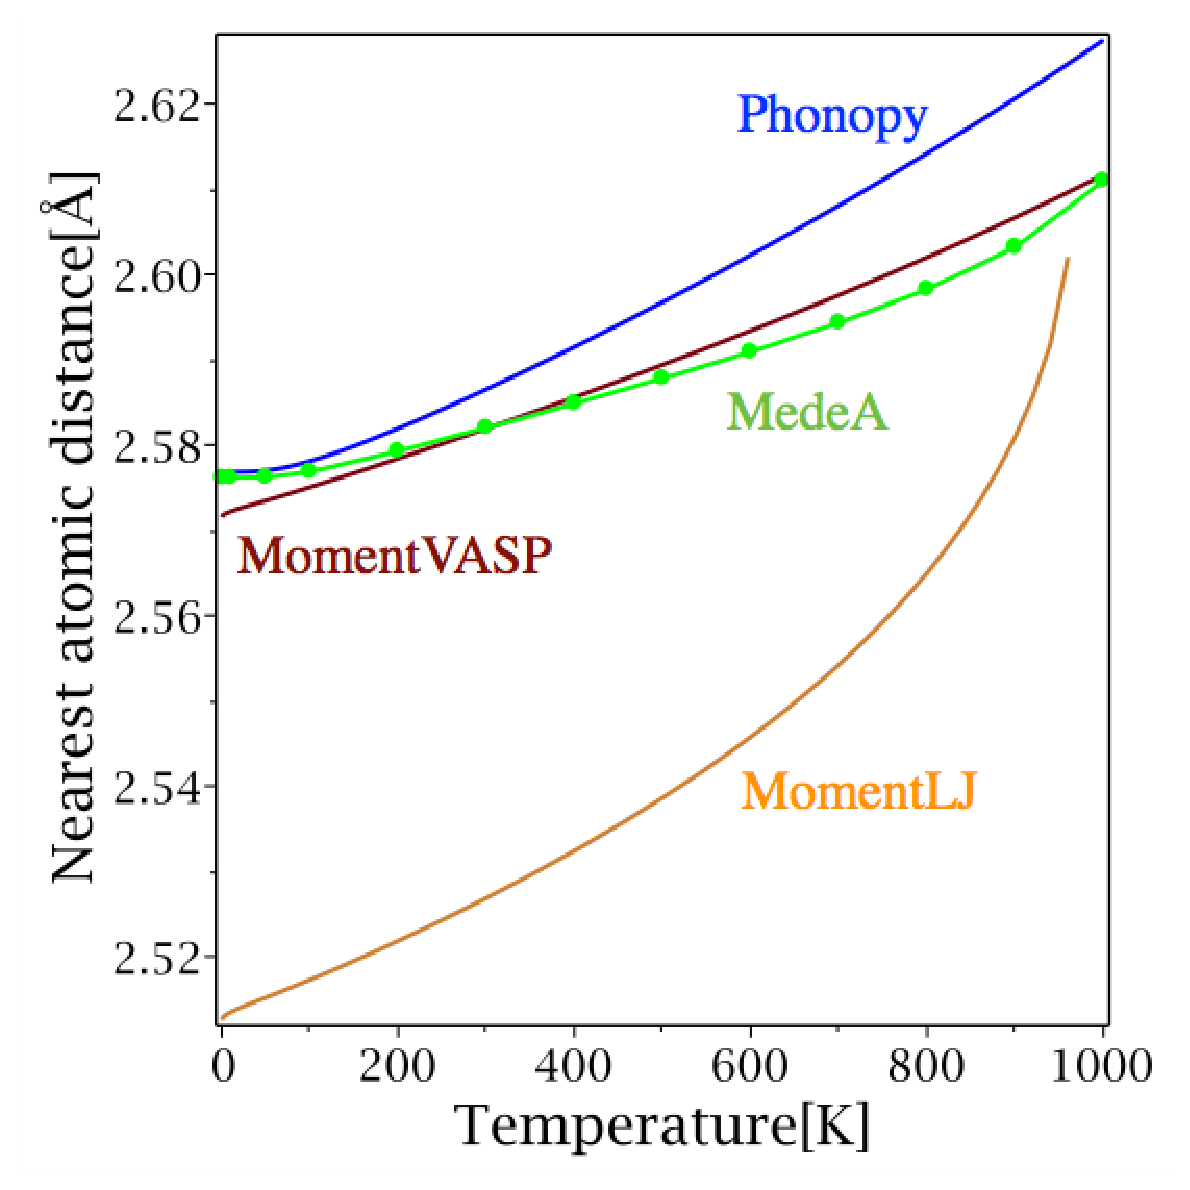
\includegraphics[keepaspectratio, scale=0.42]
  {../image_result/Cu_lat_label.eps}
  \subcaption{Cu.}\label{he1}
 \end{minipage}
 \begin{minipage}[b]{0.5\linewidth}
  \centering
  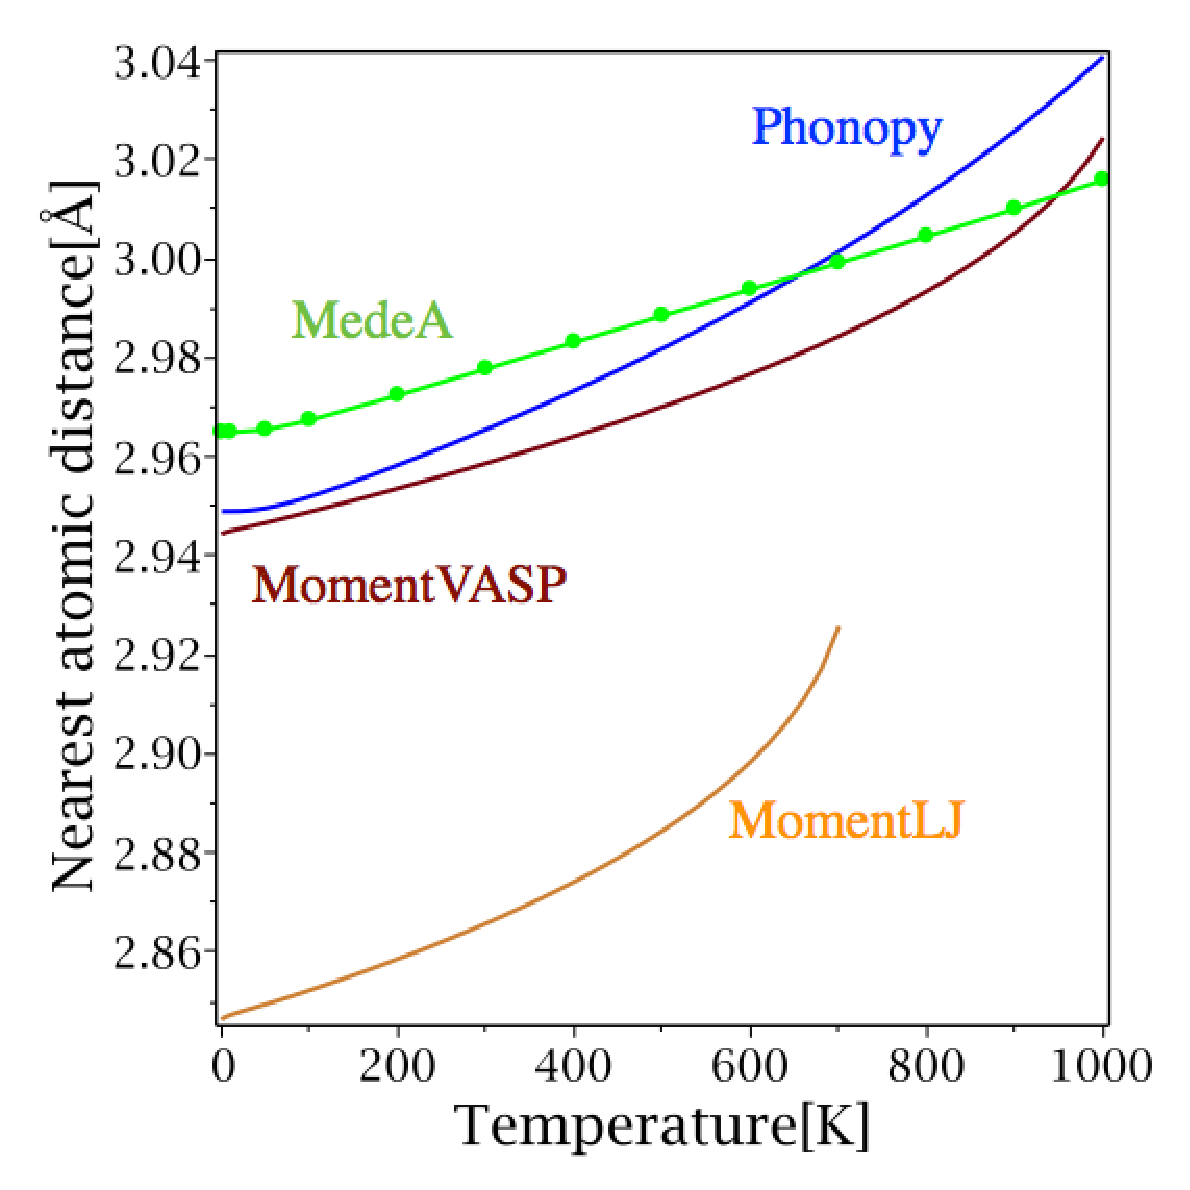
\includegraphics[keepaspectratio, scale=0.42]
  {../image_result/Ag_lat_label.eps}
  \subcaption{Ag.}\label{he2}
 \end{minipage}
 \hspace{10cm}
 \begin{minipage}[b]{0.5\linewidth}
  \centering
  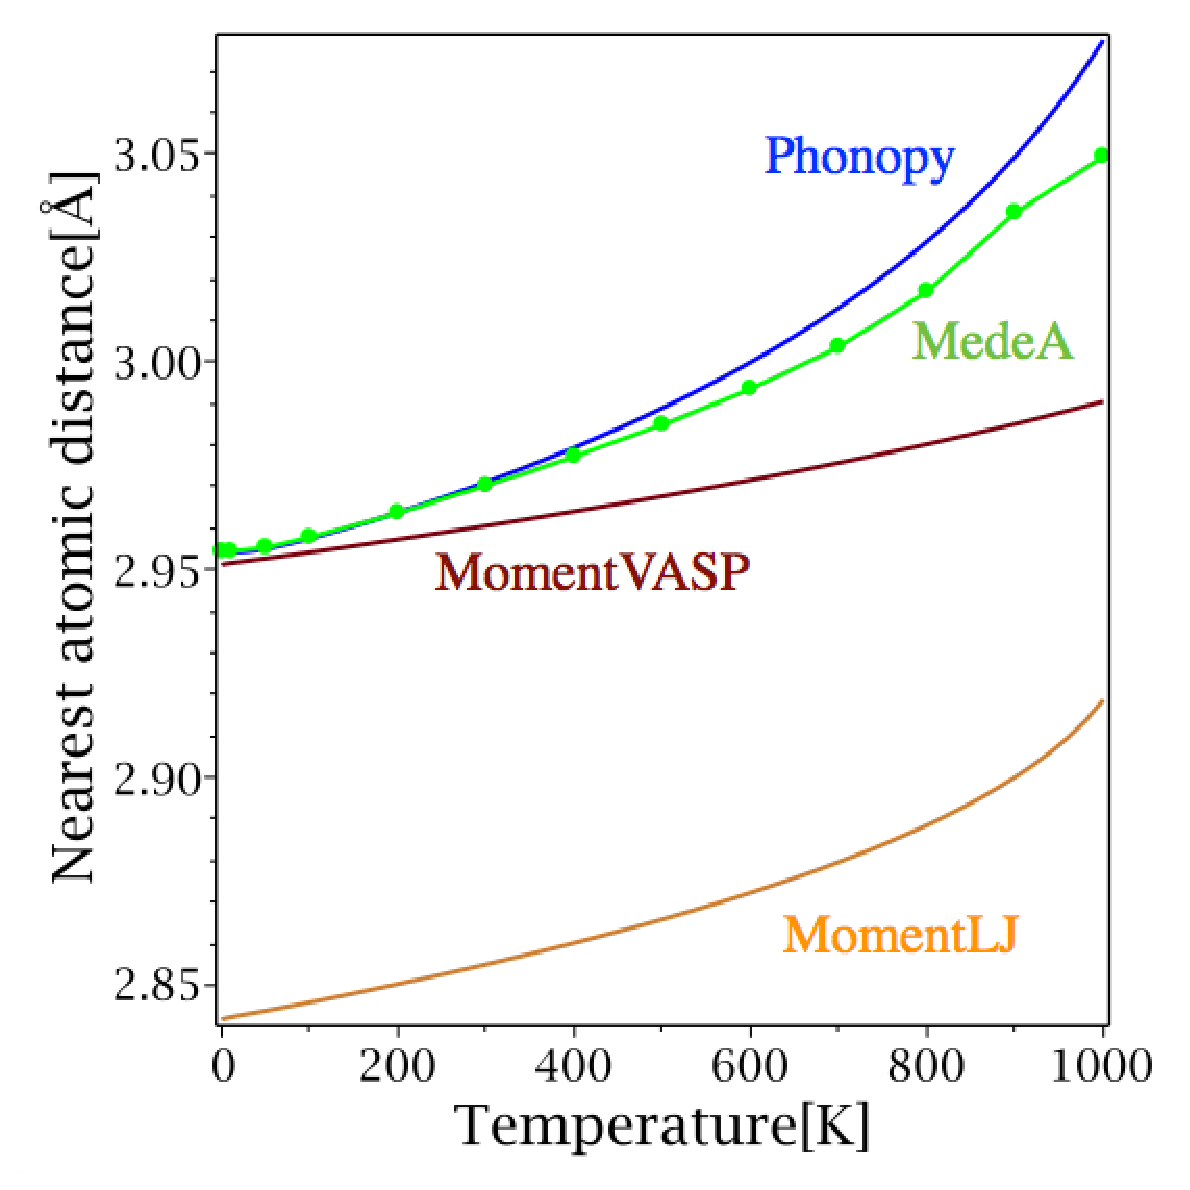
\includegraphics[keepaspectratio, scale=0.42]
  {../image_result/Au_lat_label.eps}
  \subcaption{Au.}\label{he3}
 \end{minipage}
 \begin{minipage}[b]{0.5\linewidth}
  \centering
  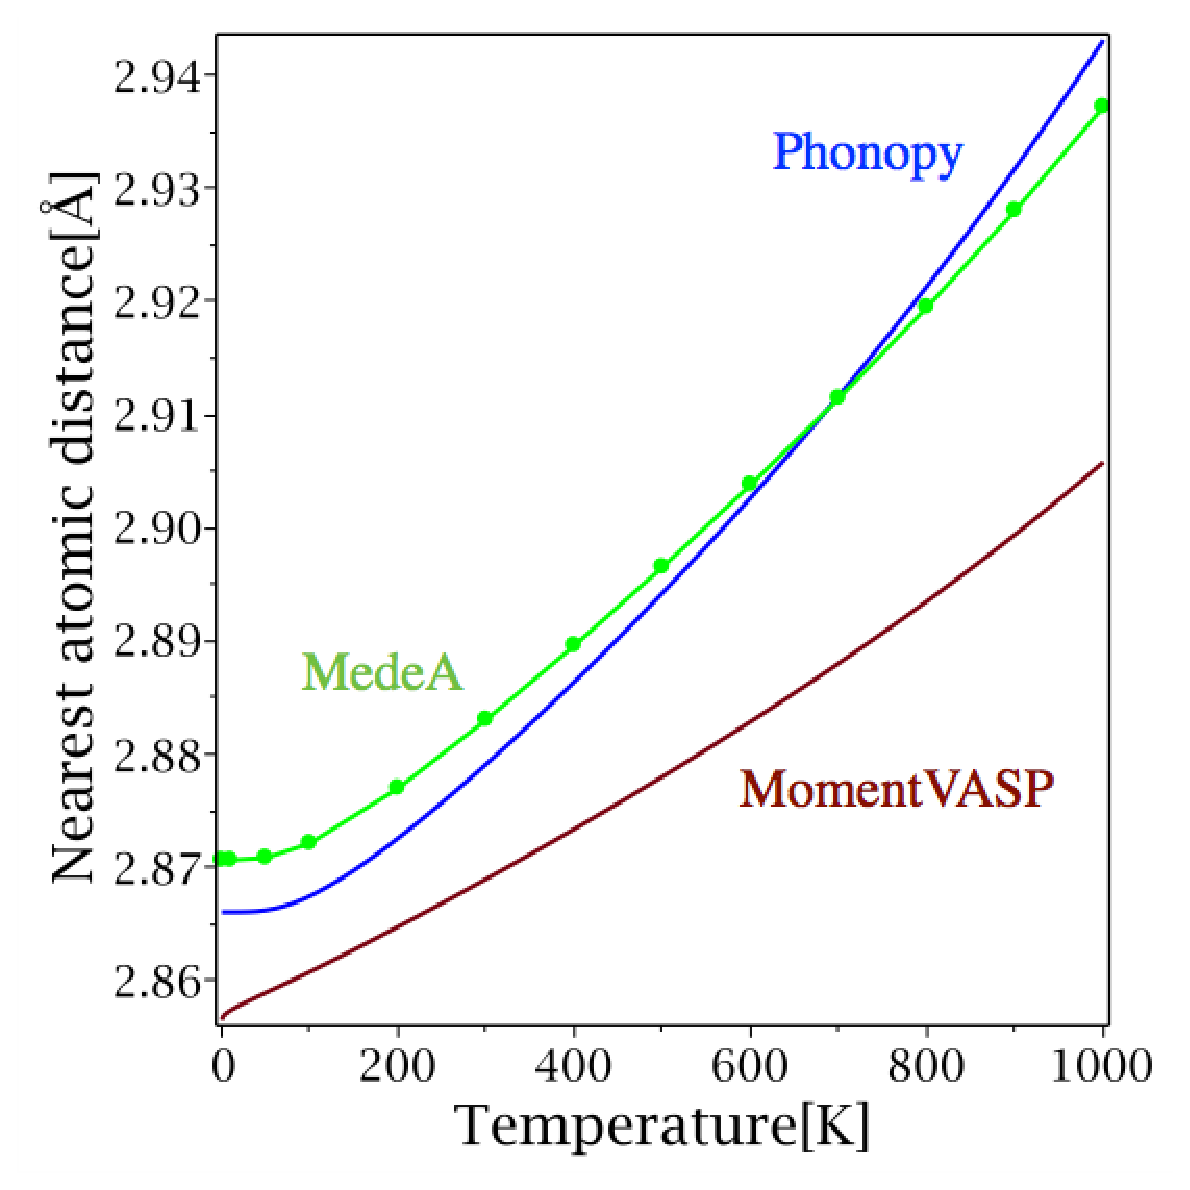
\includegraphics[keepaspectratio, scale=0.42]
  {../image_result/Al_lat_label.eps}
  \subcaption{Al.}\label{he4}
 \end{minipage}
 \caption{最近接原子間距離の温度依存性.}\label{fig:heatexpantion}
\end{figure}

\begin{figure}[htbp]
 \begin{minipage}[b]{0.5\linewidth}
  \centering
  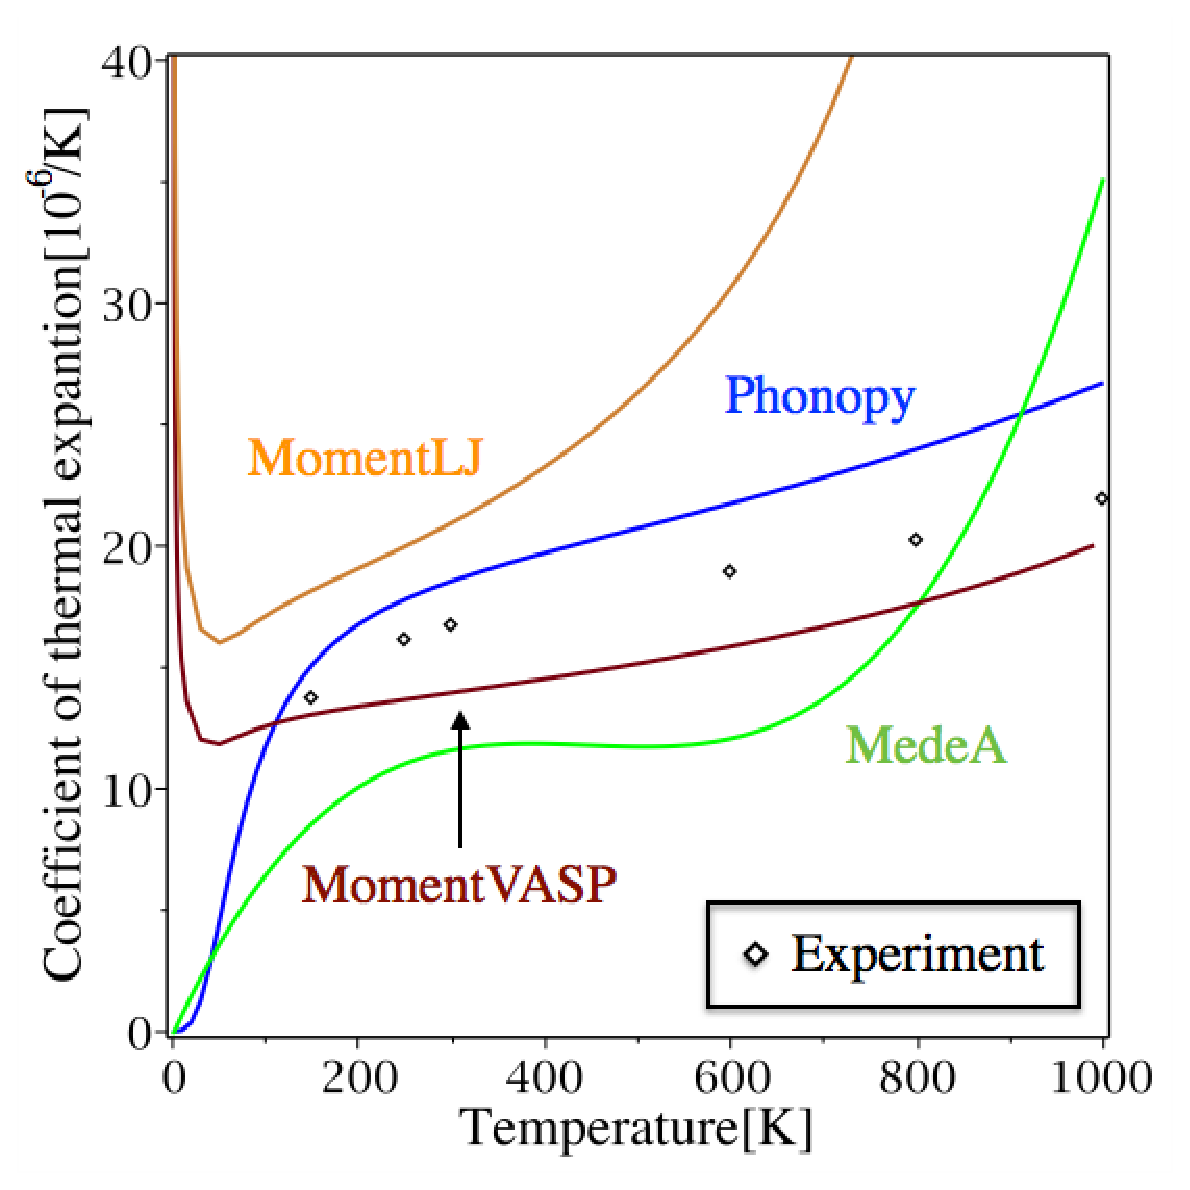
\includegraphics[keepaspectratio, scale=0.42]
  {../image_result/Cu_TEcoeff_label.eps}
  \subcaption{Cu.}\label{he5}
 \end{minipage}
 \begin{minipage}[b]{0.5\linewidth}
  \centering
  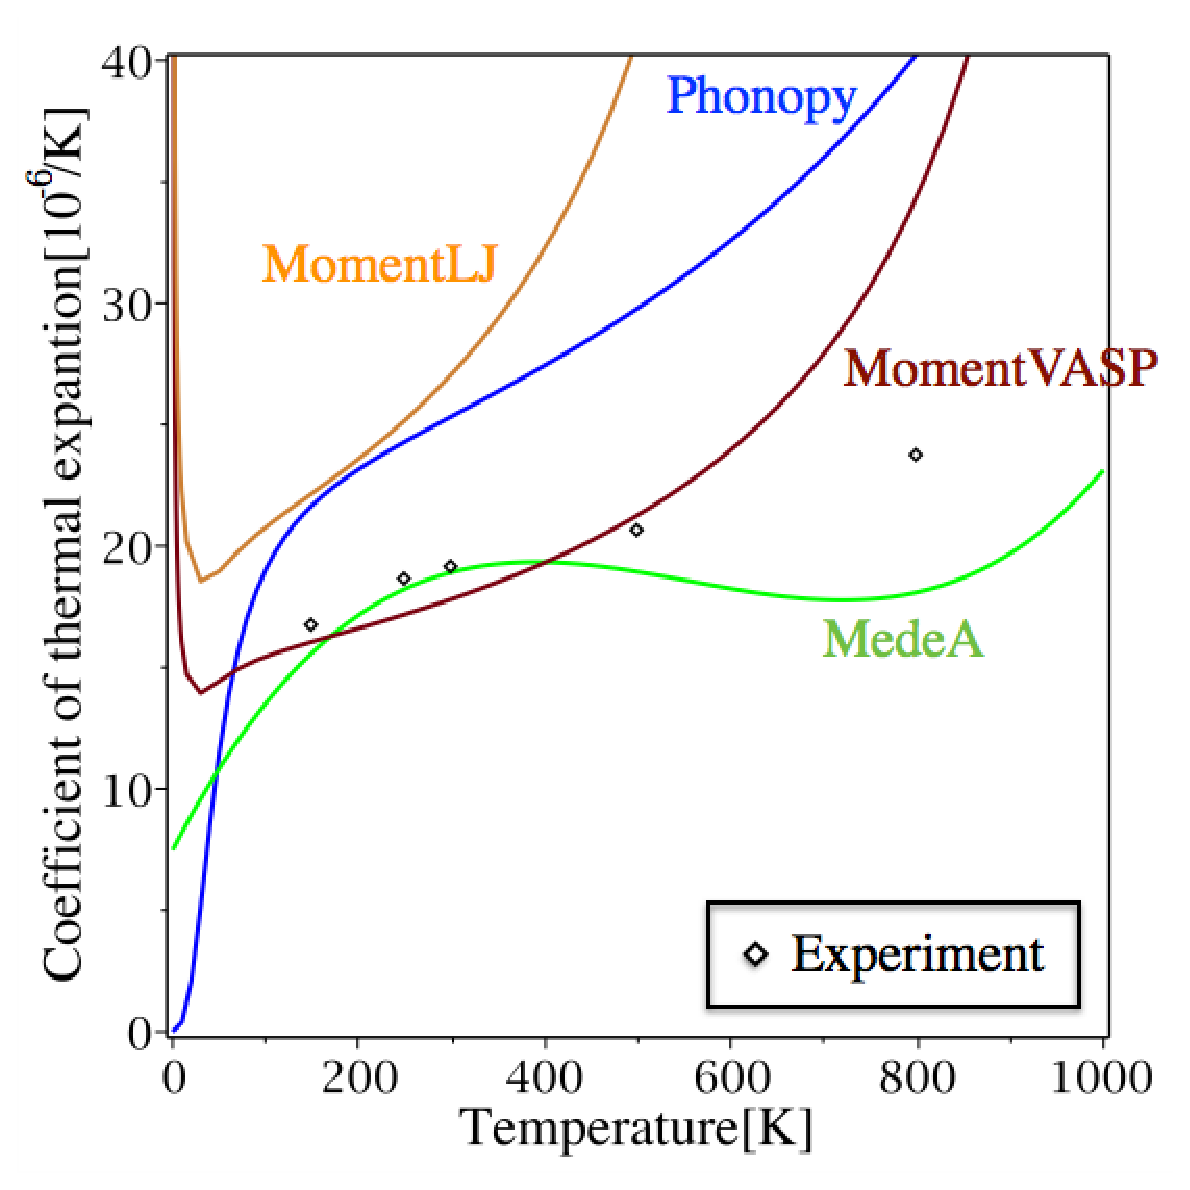
\includegraphics[keepaspectratio, scale=0.42]
  {../image_result/Ag_TEcoeff_label.eps}
  \subcaption{Ag.}\label{he6}
 \end{minipage}
 \hspace{10cm}
 \begin{minipage}[b]{0.5\linewidth}
  \centering
  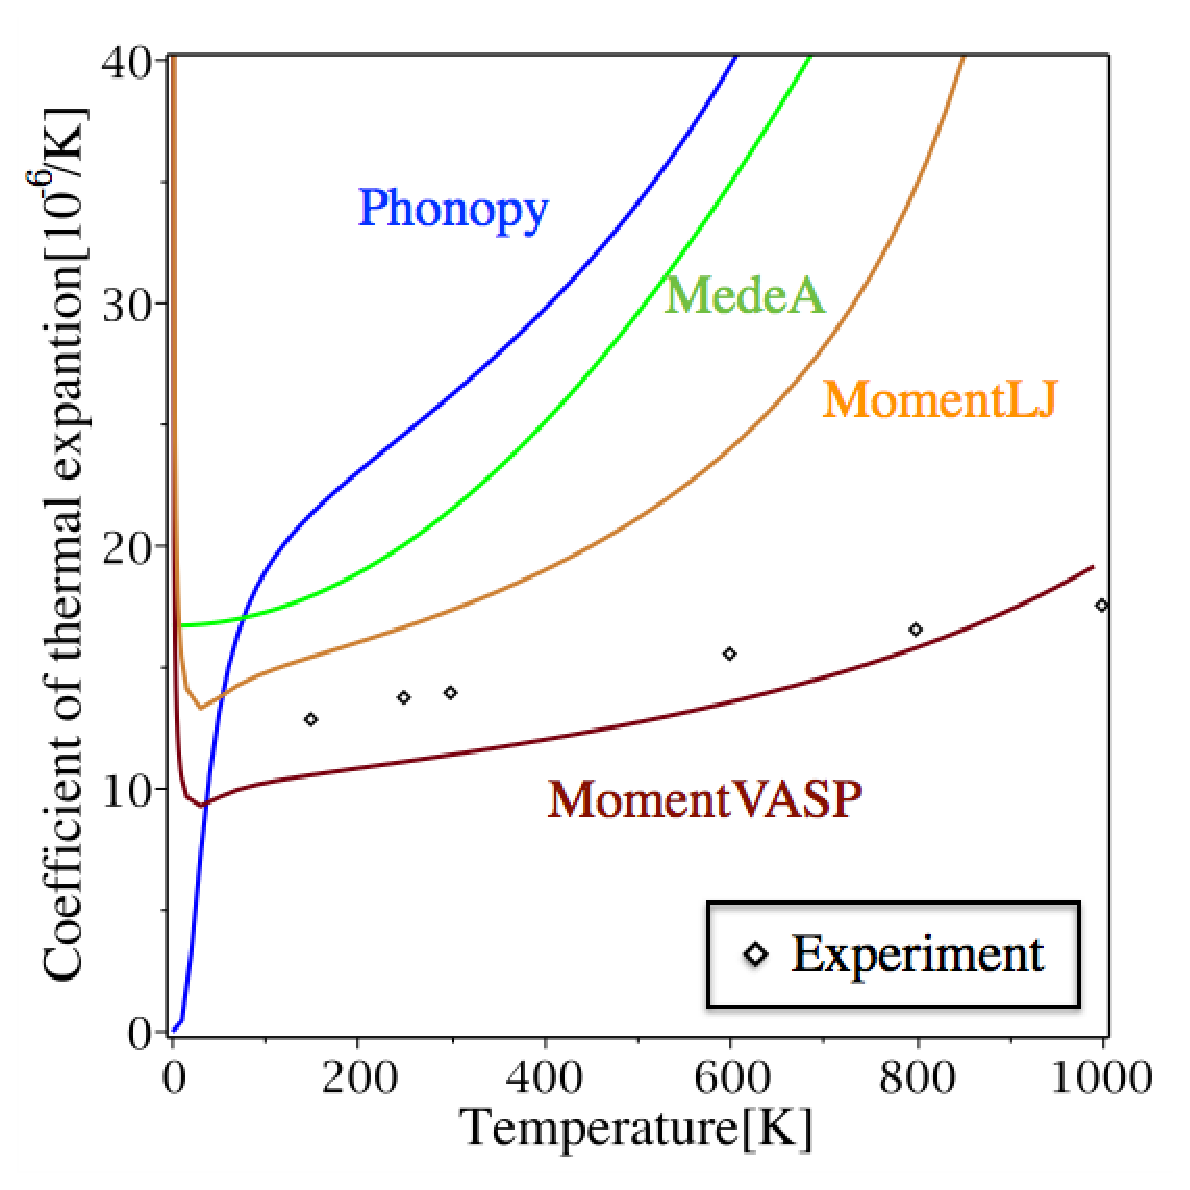
\includegraphics[keepaspectratio, scale=0.42]
  {../image_result/Au_TEcoeff_label.eps}
  \subcaption{Au.}\label{he7}
 \end{minipage}
 \begin{minipage}[b]{0.5\linewidth}
  \centering
  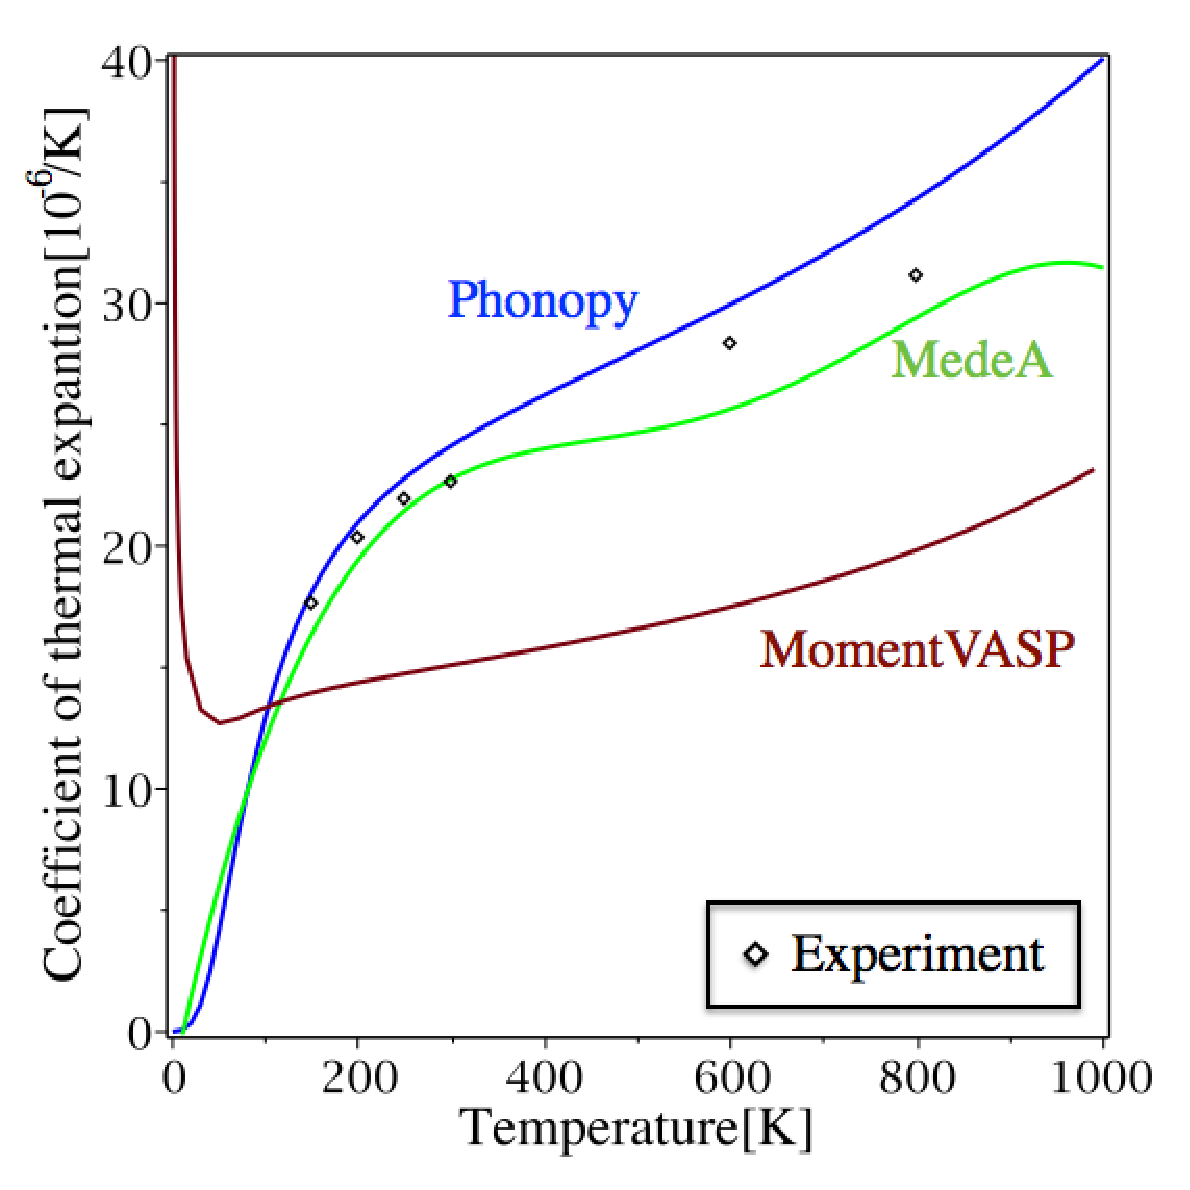
\includegraphics[keepaspectratio, scale=0.42]
  {../image_result/Al_TEcoeff_label.eps}
  \subcaption{Al.}\label{he8}
 \end{minipage}
 \caption{線膨張係数の温度依存性.}\label{fig:heatexpantion2}
\end{figure}

\section{内部エネルギー$U_0$を含まない自由エネルギー}
Medea, Phonopyの熱膨張の結果に不安があるため,まずはVASPによる構造最適化によって得られる格子定数のもとで一般的な体積一定の熱膨張を考慮していない自由エネルギーとの比較を行う.
MedeA, Phonopyによる自由エネルギーはMoment法の自由エネルギー$\psi$と比べると基底状態のエネルギーである内部エネルギー$U_0$を含んでいない.そのため$\psi$から$U_0$を消して比較を行う.結果を図\ref{fig:freeresult}に示す.この結果の0K,1000KでのMedeAとPhonopyのMomentVASPとの自由エネルギーの差を表\ref{tb:free-diff},\ref{tb:free-diff2}に示す.
MedeA, Phonopyと比べるとMomentLJ, MomentVASPともに傾きが負に大きくなっている傾向がみられる.
Moment法は熱膨張させたのちに自由エネルギーの計算をおこなっている.すなわち,最安定の自由エネルギーをとっている.
そのため,熱膨張を考慮していないMedeA,Phonopyの結果よりも値が小さくなるというのは妥当な結果だと考えられる.

\begin{figure}[htbp]
 \begin{minipage}[b]{0.5\linewidth}
  \centering
  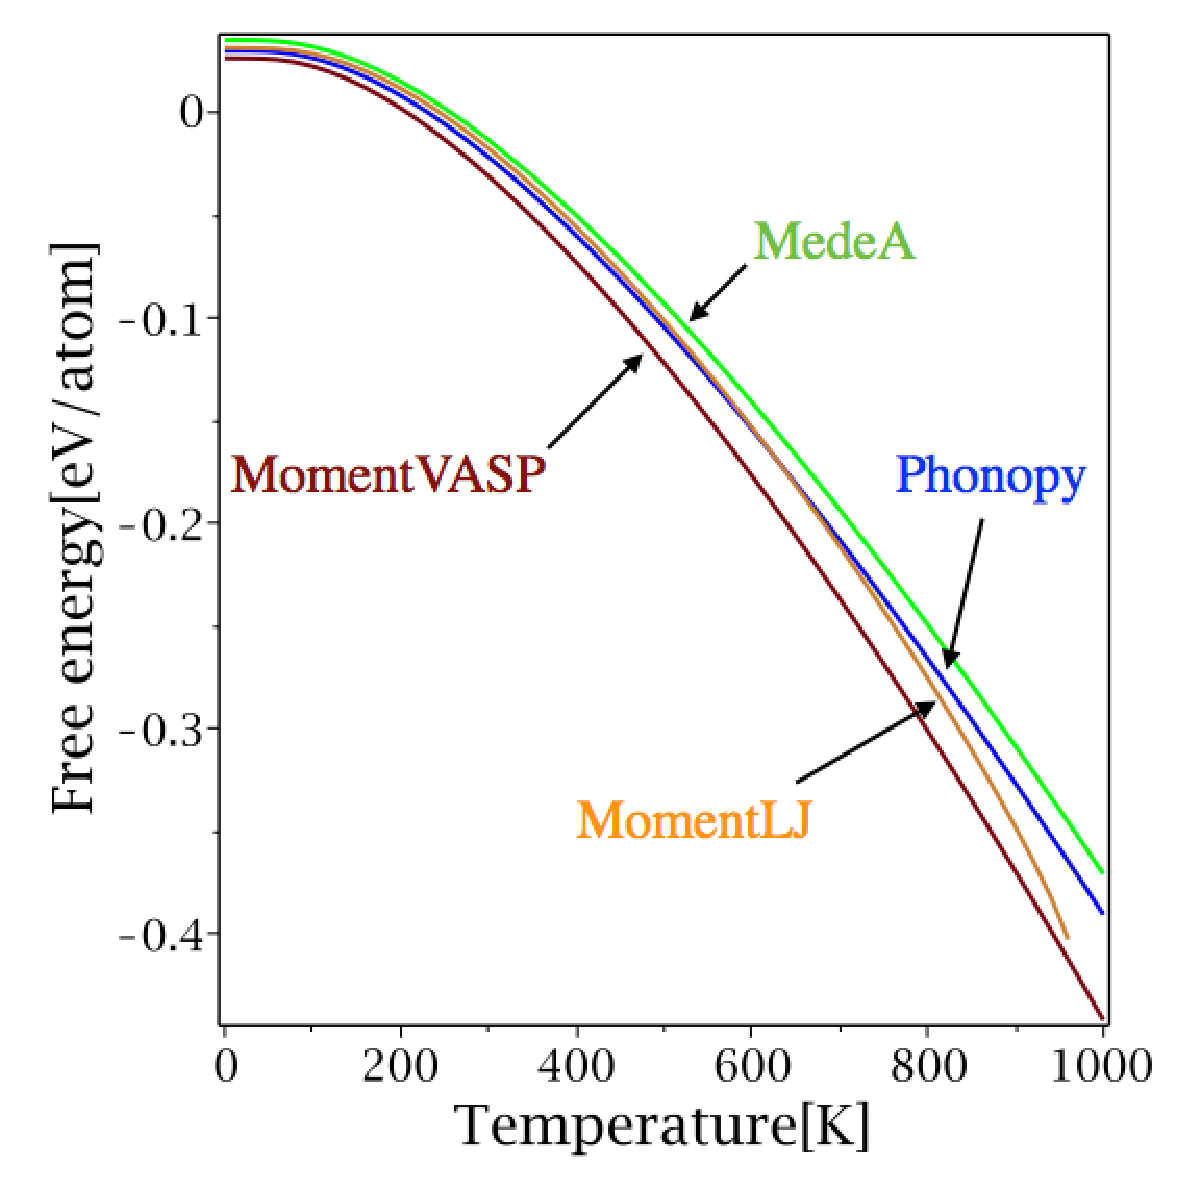
\includegraphics[keepaspectratio, scale=0.42]
  {../image_result/Cu_free_label.eps}
  \subcaption{Cu.}\label{free1}
 \end{minipage}
 \begin{minipage}[b]{0.5\linewidth}
  \centering
  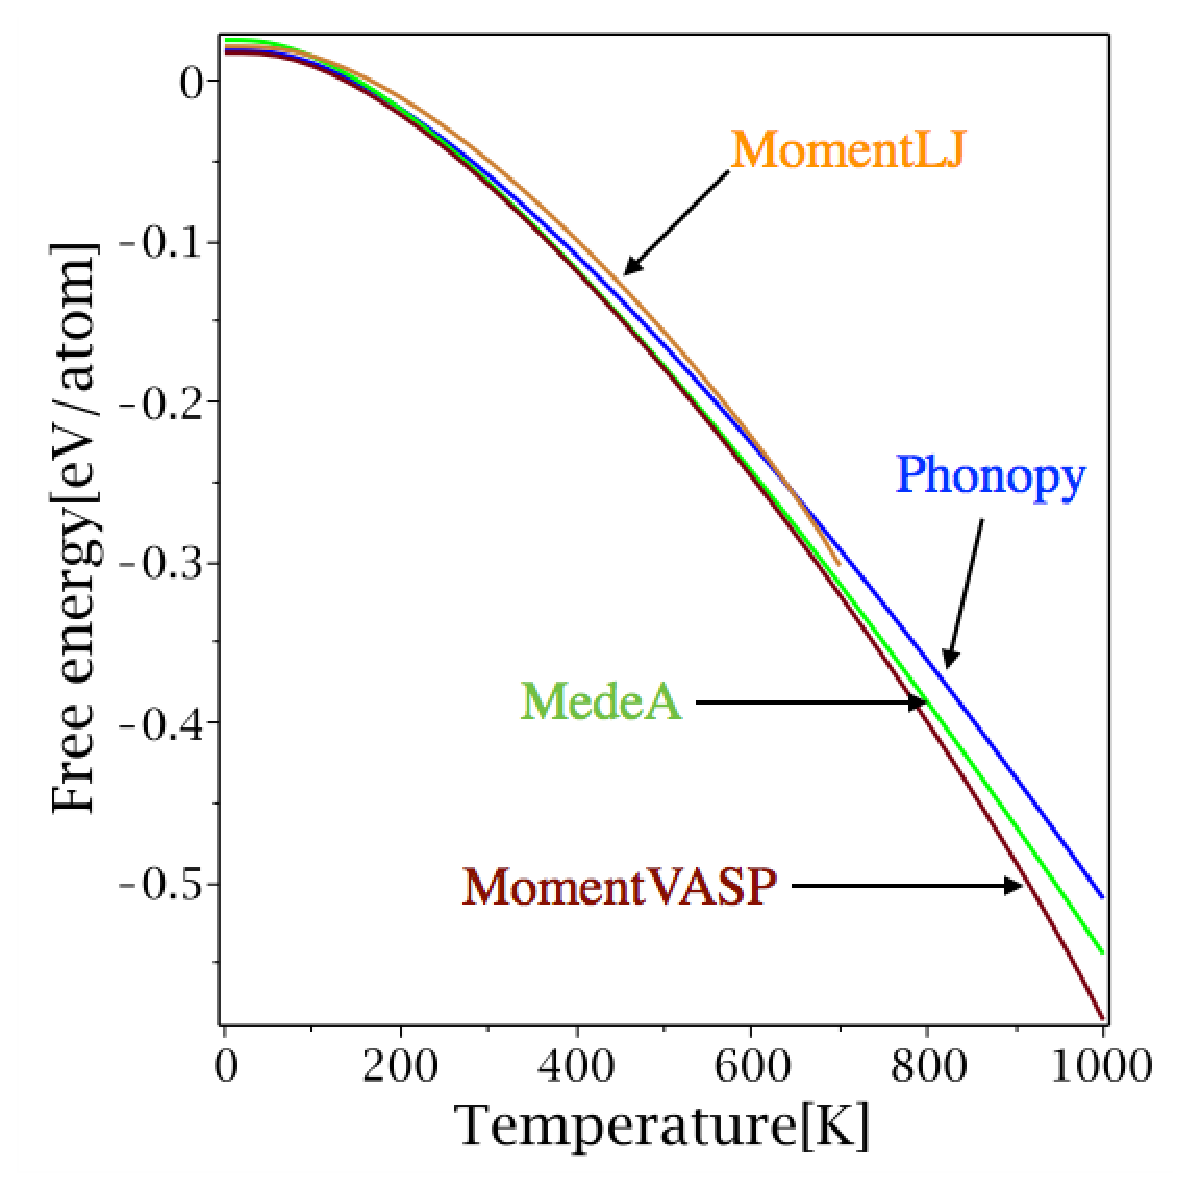
\includegraphics[keepaspectratio, scale=0.42]
  {../image_result/Ag_free_label.eps}
  \subcaption{Ag.}\label{free2}
 \end{minipage}
 \hspace{10cm}
 \begin{minipage}[b]{0.5\linewidth}
  \centering
  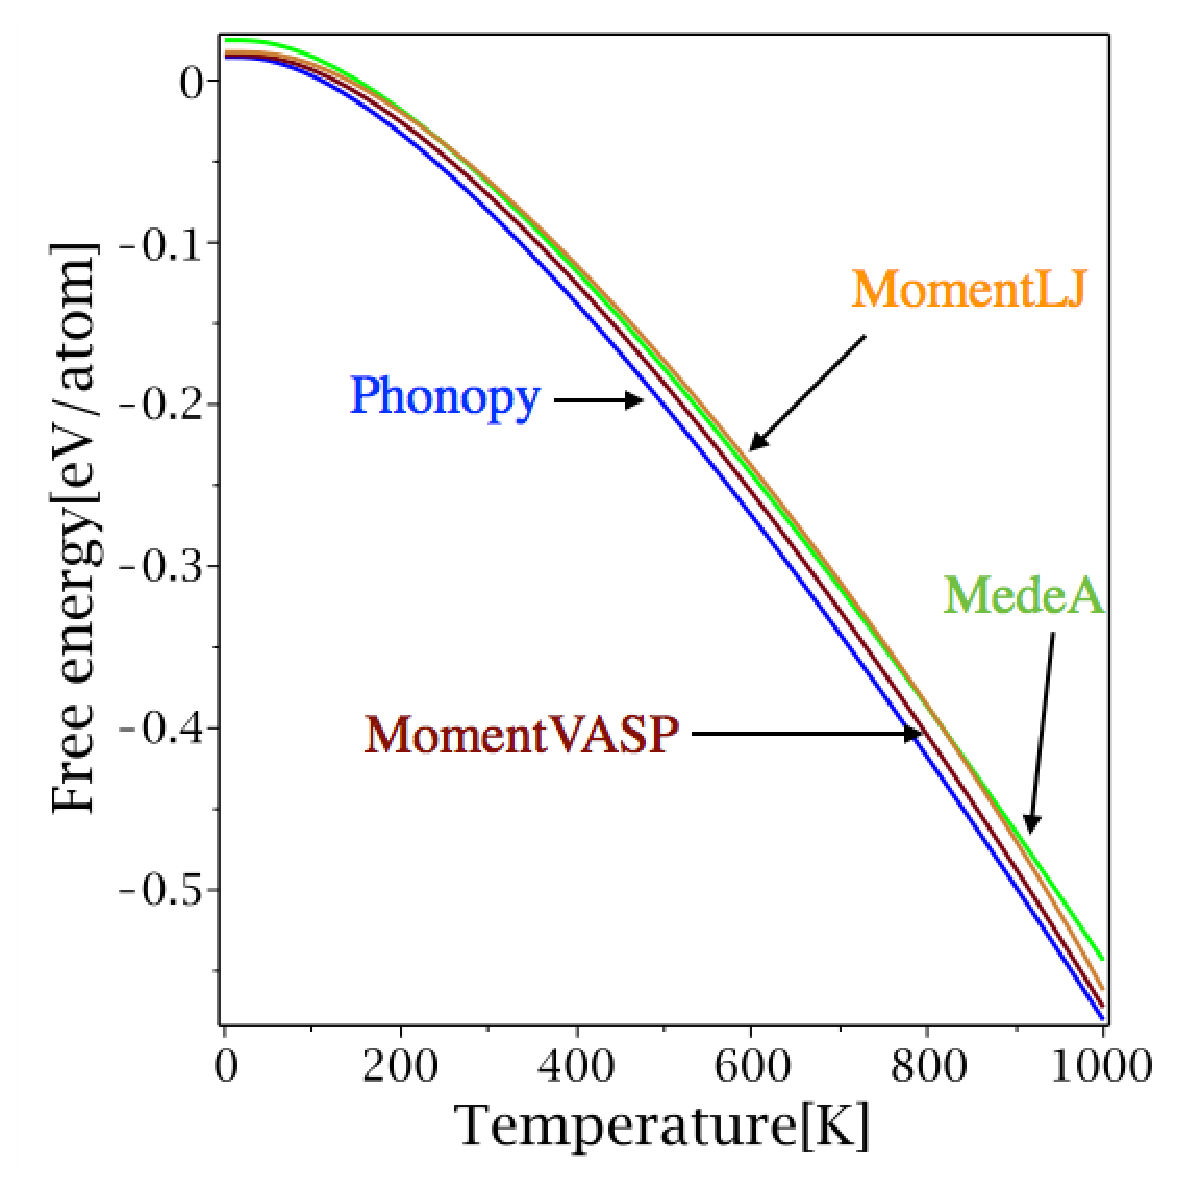
\includegraphics[keepaspectratio, scale=0.42]
  {../image_result/Au_free_label.eps}
  \subcaption{Au.}\label{free3}
 \end{minipage}
 \begin{minipage}[b]{0.5\linewidth}
  \centering
  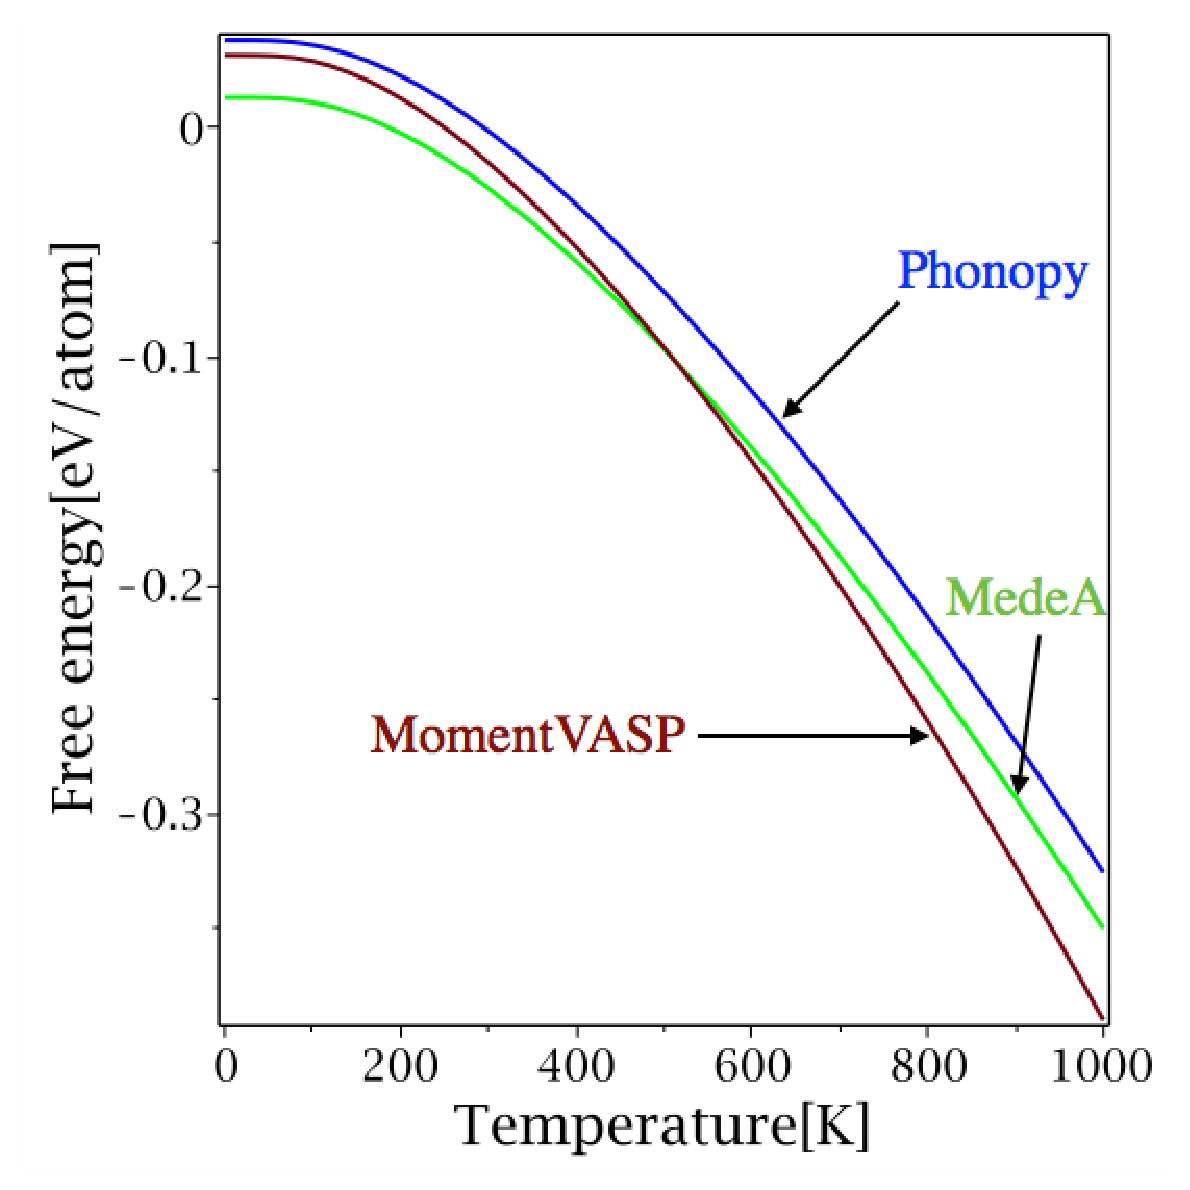
\includegraphics[keepaspectratio, scale=0.42]
  {../image_result/Al_free_label.eps}
  \subcaption{Al.}\label{free4}
 \end{minipage}
 \caption{内部エネルギー$U_0$を含まない自由エネルギーの温度依存性.MedeA, Phonopyは体積一定で計算している.}\label{fig:freeresult}
\end{figure}



\begin{table}[htbp]
  \begin{minipage}[b]{0.48\linewidth}
  \centering
  \caption{0Kと1000Kでの自由エネルギーの差(MedeA$-$MomentVASP).}
  \label{tb:free-diff}
  \begin{tabular}{ccccc}\hline
    元素 & 0K[eV] & 1000K[eV] \\ \hline \hline
    Cu & 0.008754 & 0.071124 \\
    Ag & 0.007899 & 0.041181\\
    Au & 0.009313 & 0.029068\\
    Al & -0.018484 & 0.040140\\ \hline
  \end{tabular}
 \end{minipage}
 \hspace{0.04\linewidth}
 \begin{minipage}[b]{0.48\linewidth}
 \caption{0Kと1000Kでの自由エネルギーの差(Phonopy$-$MomentVASP).}
 \label{tb:free-diff2}
  \centering
  \begin{tabular}{ccccc}\hline
    元素 & 0K[eV] & 1000K[eV] \\ \hline \hline
    Cu & 0.003605 & 0.051364  \\
    Ag & 0.001572 & 0.075705 \\
    Au & -0.001176 & -0.007870 \\
    Al & 0.006579 & 0.064626 \\ \hline
  \end{tabular}
 \end{minipage}
\end{table}




\section{内部エネルギー$U_0$を含んだ自由エネルギー}
次にPhonopyによる内部エネルギー$U_0$と熱膨張を考慮に入れた自由エネルギーとの比較を\ref{fig:freeresult2}に示す.この結果の0K,1000KでのPhonopyとMomentVASPとの自由エネルギーの差を表\ref{tb:free-diff3}に示す.
先ほどの図\ref{fig:freeresult}の結果と比べると,内部エネルギーと熱膨張を考慮に入れたことによってPhonopyの傾きがMomentVASPに近づいている.また,表\ref{tb:free-diff2}と\ref{tb:free-diff3}の自由エネルギーの差を見比べると4元素全ての値の差が小さくなっている.
特にCu, AgはAu, Alと比較すると値がよく一致している.これは図\ref{heatexpantion}のCu, Agの熱膨張の結果がAu, Alよりも近い数字を出しているからだと考えられる.
この結果はMoment法は熱膨張の効果を取り入れた自由エネルギーの計算をPhonopyと同等程度に行えていることを示唆している.

\begin{figure}[htbp]
 \begin{minipage}[b]{0.5\linewidth}
  \centering
  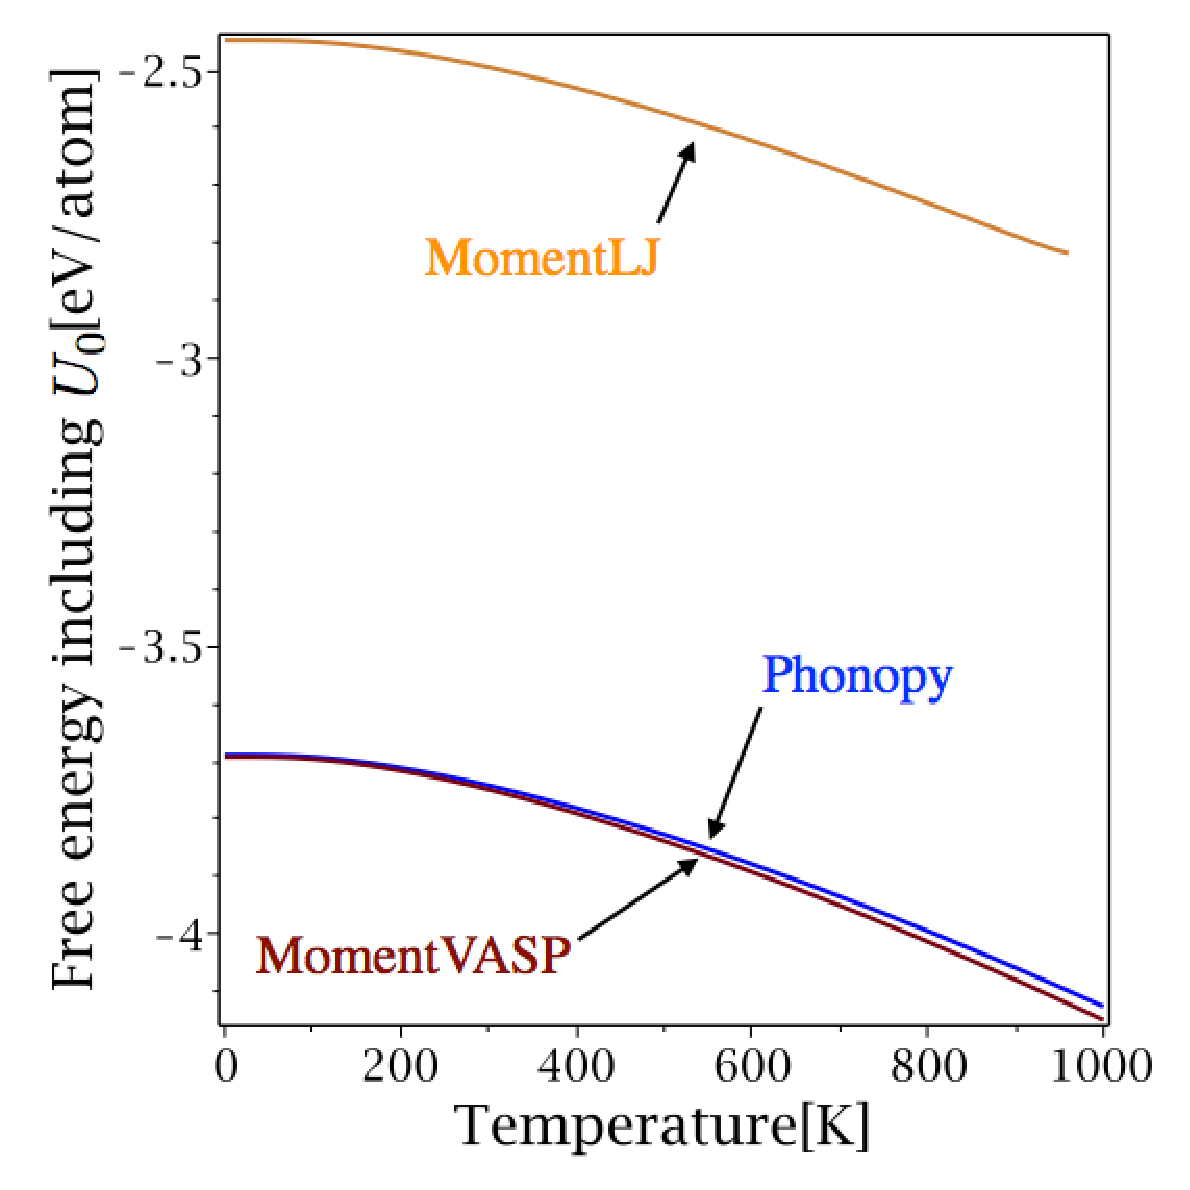
\includegraphics[keepaspectratio, scale=0.42]
  {../image_result/Cu_free_u0_label.eps}
  \subcaption{Cu.}\label{free5}
 \end{minipage}
 \begin{minipage}[b]{0.5\linewidth}
  \centering
  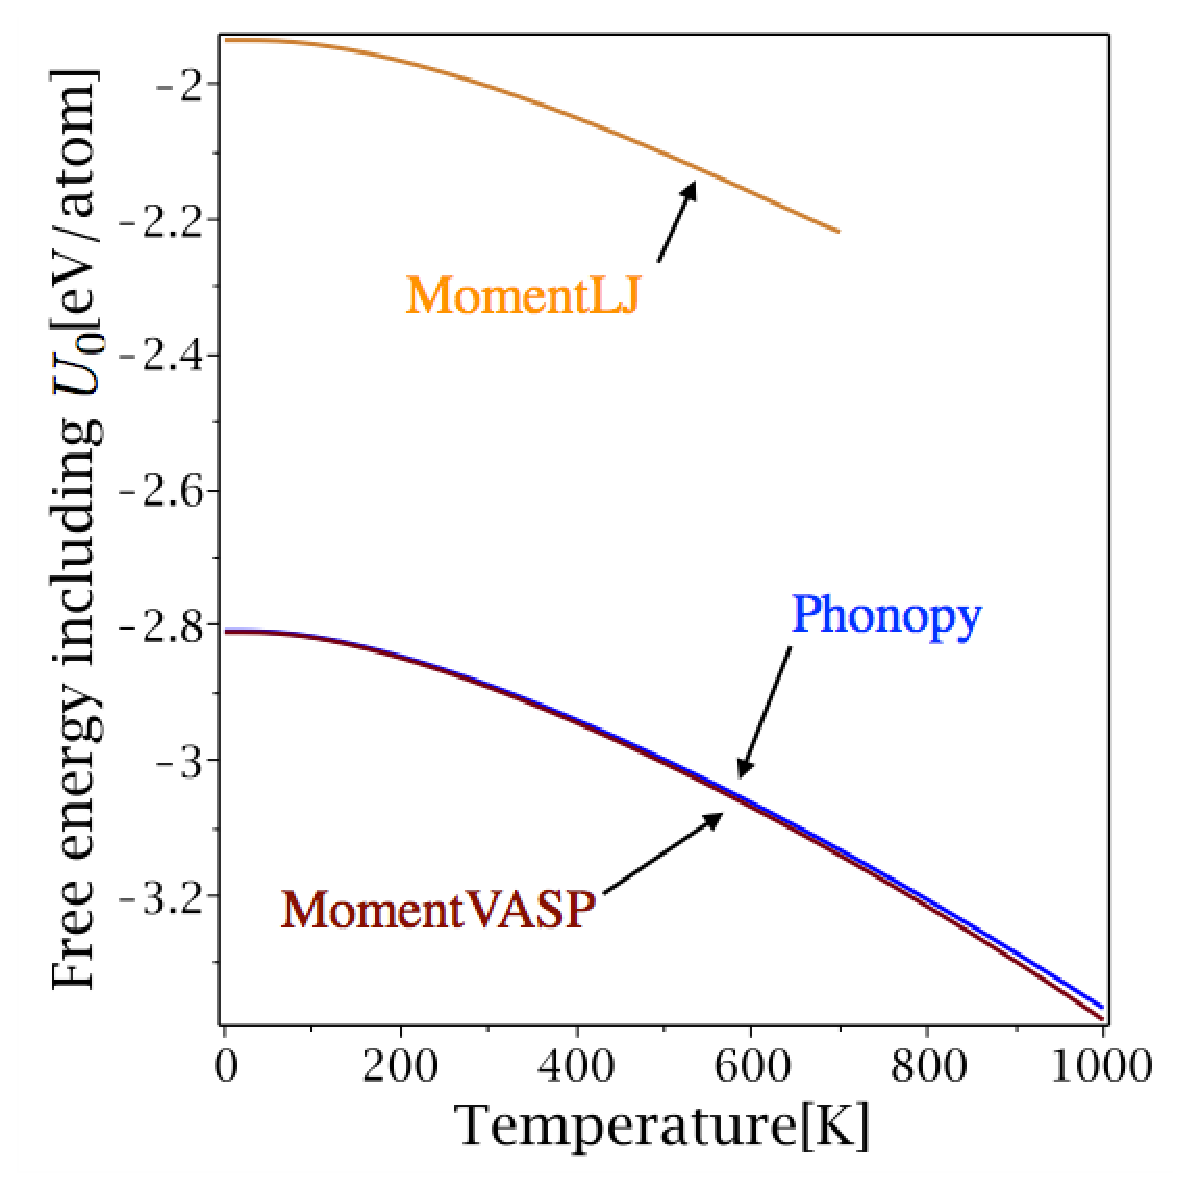
\includegraphics[keepaspectratio, scale=0.42]
  {../image_result/Ag_free_u0_label.eps}
  \subcaption{Ag.}\label{free6}
 \end{minipage}
 \hspace{10cm}
 \begin{minipage}[b]{0.5\linewidth}
  \centering
  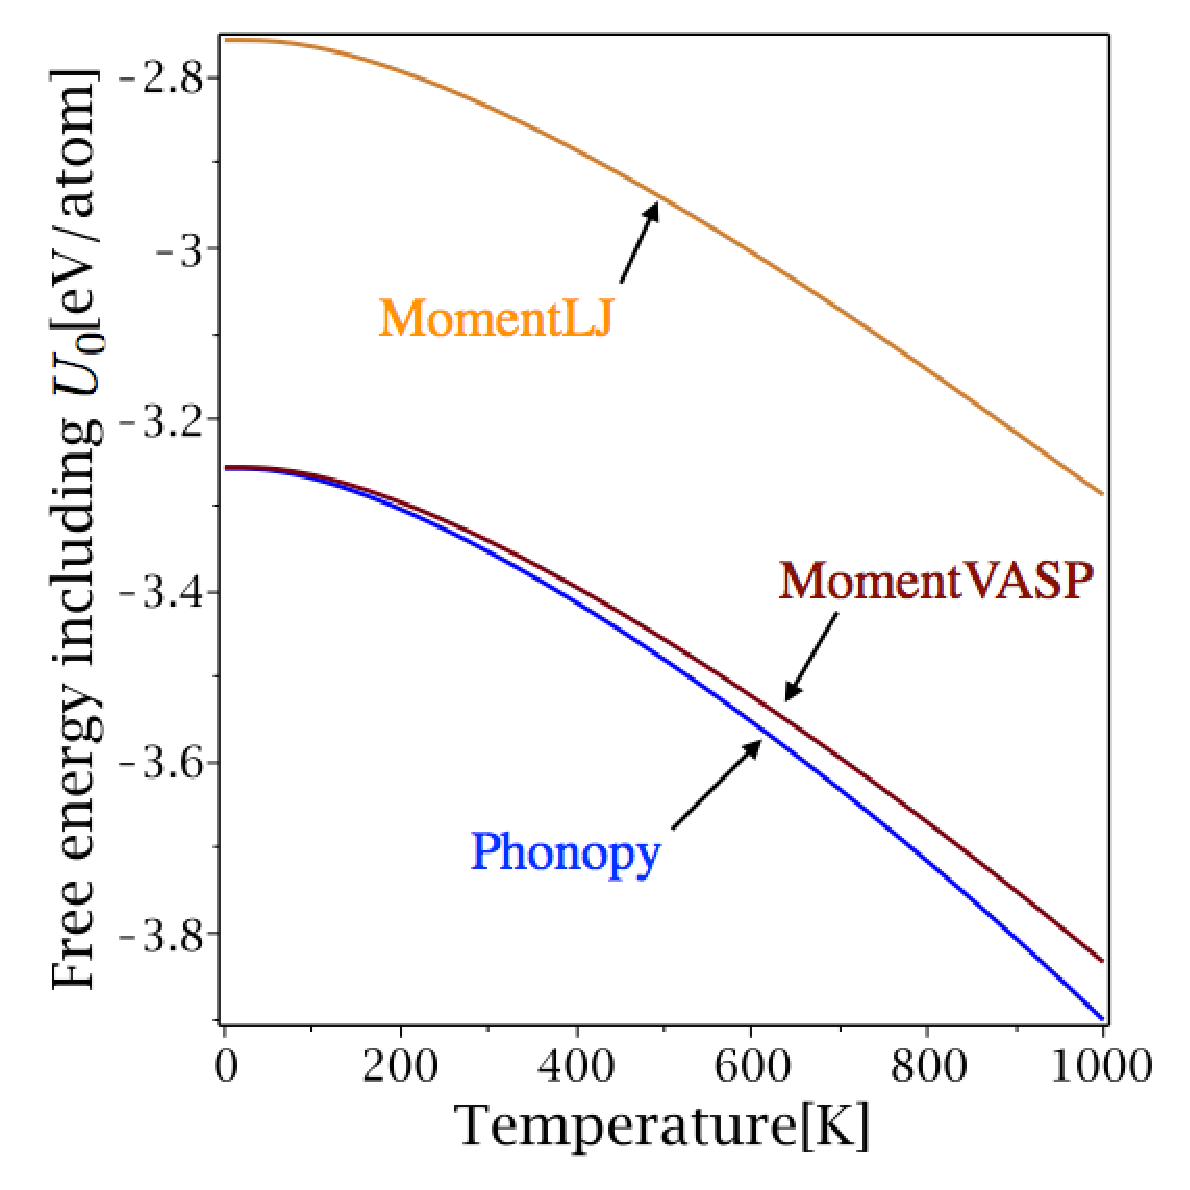
\includegraphics[keepaspectratio, scale=0.42]
  {../image_result/Au_free_u0_label.eps}
  \subcaption{Au.}\label{free7}
 \end{minipage}
 \begin{minipage}[b]{0.5\linewidth}
  \centering
  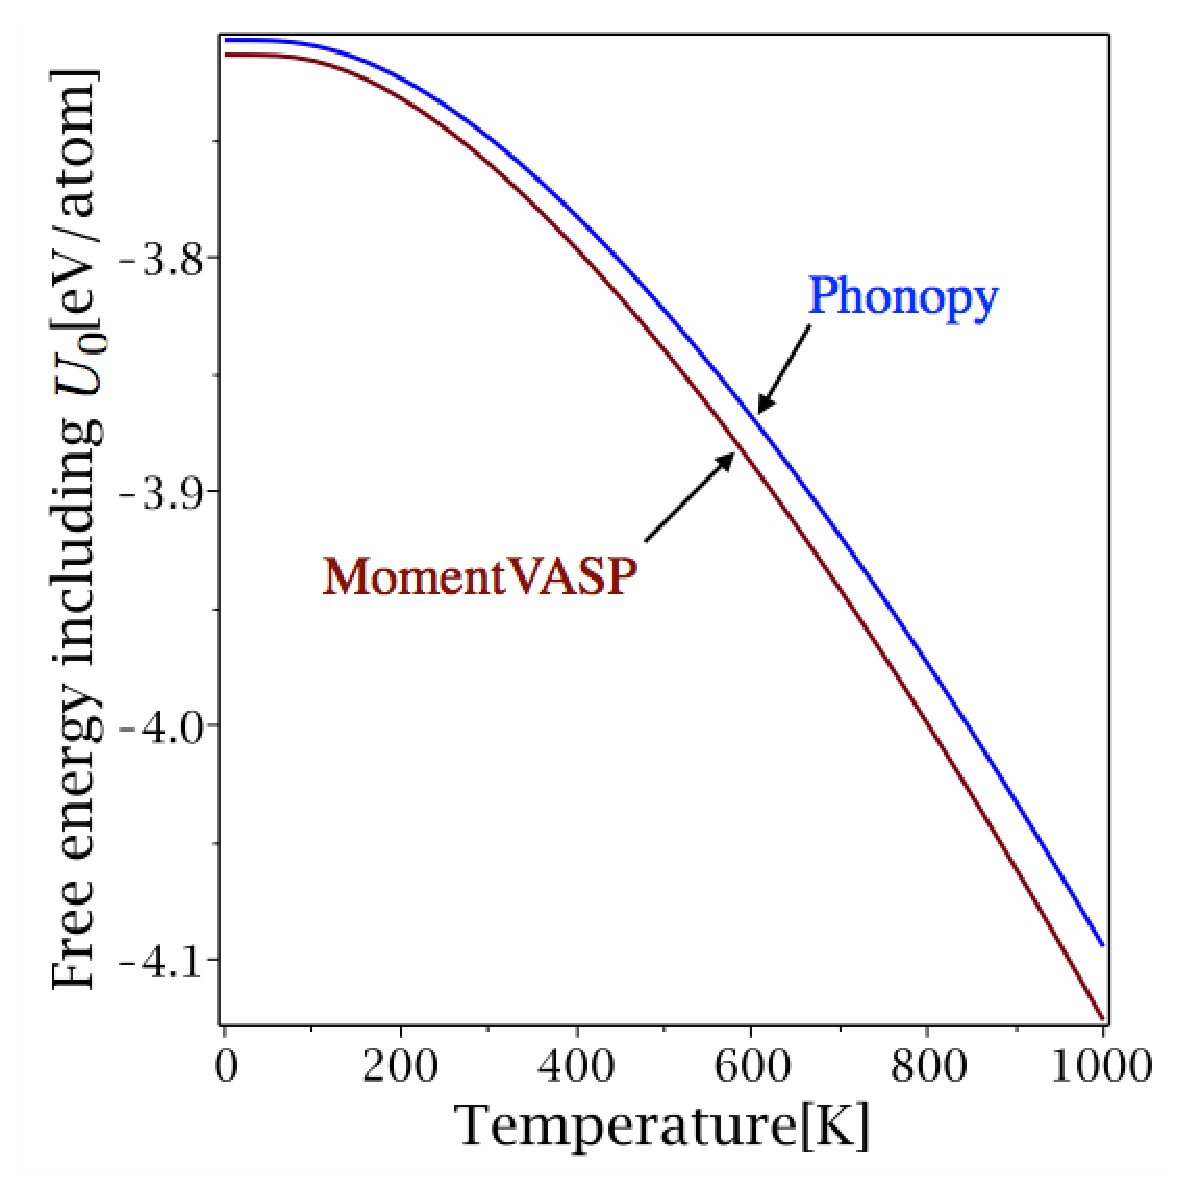
\includegraphics[keepaspectratio, scale=0.42]
  {../image_result/Al_free_u0_label.eps}
  \subcaption{Al.}\label{free8}
 \end{minipage}
 \caption{内部エネルギー$U_0$を含んだ自由エネルギーの温度依存性.Phonopyは$U_0$と熱膨張を考慮に入れて計算している.}\label{fig:freeresult2}
\end{figure}

\begin{table}[htbp]
\caption{0Kと1000Kでの$U_0$を考慮に入れた自由エネルギーの差(Phonopy$-$MomentVASP)}
  \label{tb:free-diff3}
  \centering
  \begin{tabular}{ccccc}\hline
    元素 & 0K[eV] & 1000K[eV] \\ \hline \hline
    Cu & 0.003348 & 0.023715 \\
    Ag & 0.001408 & 0.017776 \\
    Au & -0.00124 & -0.06791 \\
    Al & 0.006197 & 0.031391 \\ \hline
  \end{tabular}
\end{table}
%結果
\chapter{考察}
\section{低温域の熱膨張について}
\label{sec:he_100k}
Moment法の熱膨張の結果は低温域で現実的ではない値を見積もっている.
原因を$y_0$の関数から考える.まず式(\ref{eq:moment15})より$y_0$は
\begin{eqnarray}
\label{eq:y01}
y_0= \sqrt{\frac{2\gamma\theta^2}{3k^3}A}
\end{eqnarray}
であり,$\theta=k_{\rm{B}}T$を代入し,
\begin{eqnarray}
\label{eq:y02}
y_0= \sqrt{\frac{2\gamma(k_{\rm{B}}T)^2}{3k^3}A}
\end{eqnarray}
と書ける.これを変形すると$y_0$は
\begin{eqnarray}
\label{eq:y02}
y_0= \sqrt{\frac{2\gamma}{3k^3}}k_{\rm{B}}\times \sqrt{A} \times T
\end{eqnarray}
このように書くことができる.
$\sqrt{\frac{2\gamma}{3k^3}}k_{\rm{B}}$は$k$,$\gamma$の関数であり原子間距離によって値が定まる.Cuのペアポテンシャルの$k$, $\gamma$による,最近接原子間距離と$\sqrt{\frac{2\gamma}{3k^3}}k_{\rm{B}}$の関係を図\ref{fig:y0_heat}(\subref{y0_heat1})に示す.
また,$\sqrt{A}$は$k$, $\gamma$, $T$の関数であり,簡単な2次元のグラフでは表すことができない.
しかし,実際の熱膨張の計算結果に用いられた$\sqrt{A}$の数値を見れば取り得る値の範囲がわかり傾向を掴むことができる.
それを図\ref{fig:y0_heat}(\subref{y0_heat2})に示す.
(\subref{y0_heat1})より$\sqrt{\frac{2\gamma}{3k^3}}k_{\rm{B}}$は原子間距離に対して緩やかなカーブを描きながら増加しており,低温域の急激な熱膨張には影響していないことがわかる.
また,(\subref{y0_heat1})からは,$\sqrt{A}$は,1Kから50Kにかけて急激に減少しており,逆に低温域での熱膨張を抑えていることがわかる.最後に$y_0$の残りの成分である$T$に着目すると,単純に1Kから100Kの温度変化で$y_0$を100倍していることになり,これは明らかに低温域の急激な熱膨張の原因だとわかる.これらの結果からMoment法の低温域での急激な熱膨張は,$y_0$に含まれる$T$が原因であり,$T$の増加率,実際の計算結果から考えると100K以下の結果は参考にならないと言える.
\begin{figure}[htbp]
 \begin{minipage}[b]{0.5\linewidth}
  \centering
  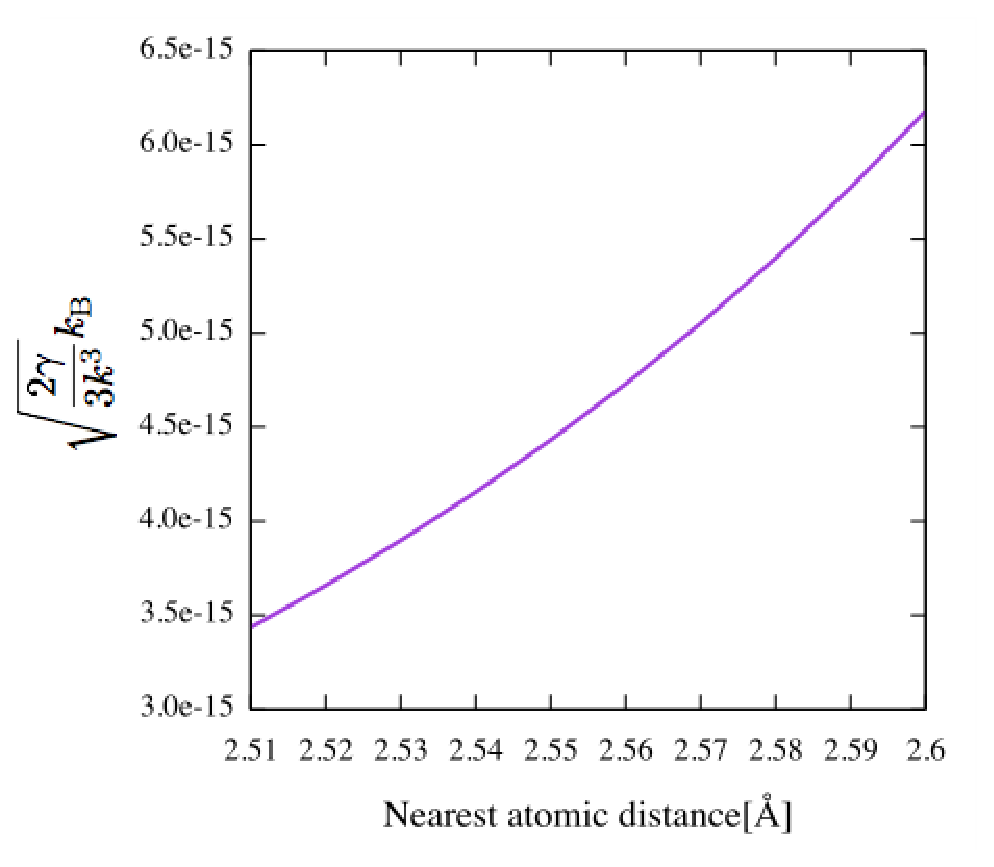
\includegraphics[keepaspectratio, scale=0.42]
  {../image/y0_no_largea_label.eps}
  \subcaption{}\label{y0_heat1}
 \end{minipage}
 \begin{minipage}[b]{0.5\linewidth}
  \centering
  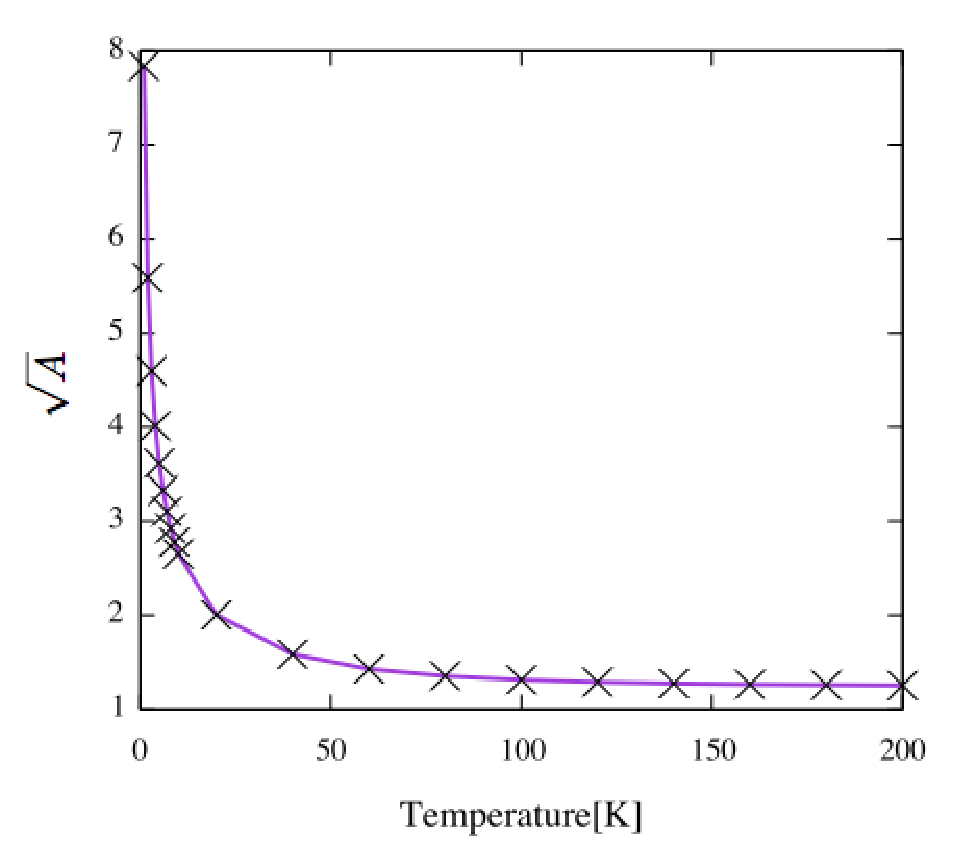
\includegraphics[keepaspectratio, scale=0.42]
  {../image/y0_largea_label.eps}
  \subcaption{}\label{y0_heat2}
 \end{minipage}
 \caption{$y_0$に含まれる関数の概形.
 (\subref{y0_heat1})は$\sqrt{\frac{2\gamma}{3k^3}}k_{\rm{B}}$は$k$,$\gamma$と原子間距離の関係,(\subref{y0_heat1})は実際の各温度での熱膨張計算で$\sqrt{A}$ が取る値を示している.$k$, $\gamma$にはCuのペアポテンシャルを用いた.
 }\label{fig:y0_heat}
\end{figure}

\section{$a_0$を変えた計算結果}
熱膨張の計算における0Kでの原子間距離に着目していく.
MomentVASPの計算は最近接原子間距離の初期値である$a_0$にVASPの構造最適化による最安定距離を使用している.それに比べMedeA, Phonopyは振動による自由エネルギーを考慮しているため0Kでの格子の長さは基底状態とは異なってくる.
例えばAlであれば0KにおけるMomentVASPの最近接原子間距離は2.856$\mathrm{\AA}$, Phonopyは2.866$\mathrm{\AA}$であり,その差は0.01$\mathrm{\AA}$ある.Moment法は$a_0$の値を変えると$k$, $\gamma$を参照する$y$の値が変わり違う結果を出してくれる.
そこで,MomentVASPの計算に使用していた$a_0$をPhonopyの0Kの原子間距離に変えることによって,結果が改善されるのではないかと考えた.
Alによる結果を図\ref{fig:a0test}に示す.

\begin{figure}[htbp]
 \begin{minipage}[b]{0.5\linewidth}
  \centering
  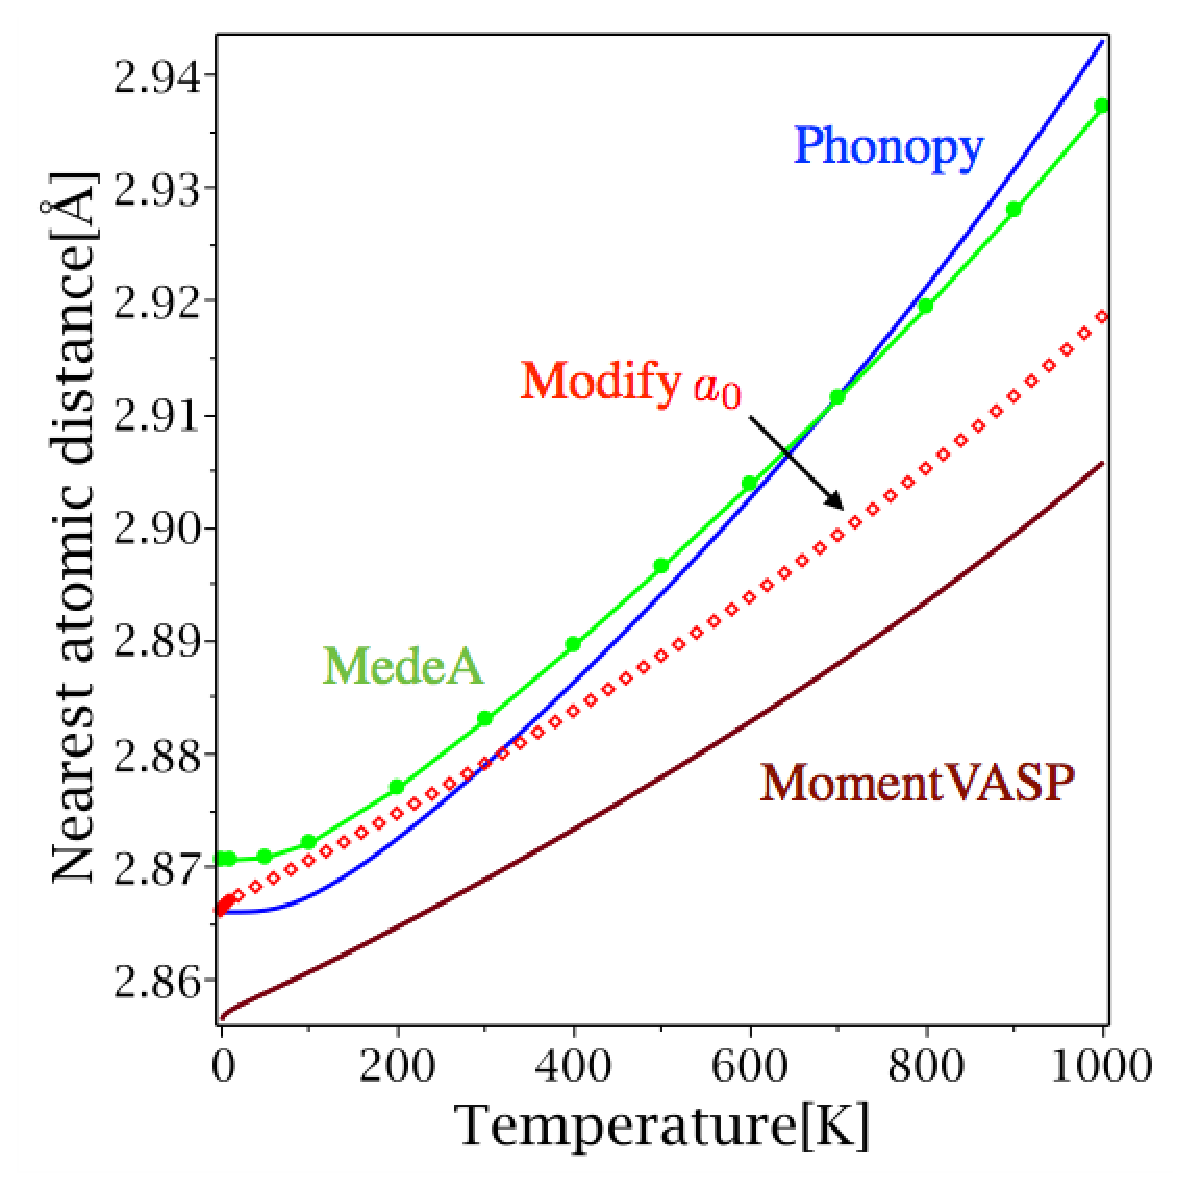
\includegraphics[keepaspectratio, scale=0.42]
  {../image_result/Al_lat_phonopy_label.eps}
  \subcaption{最近接原子間距離と温度の依存性}\label{a0test1}
 \end{minipage}
 \begin{minipage}[b]{0.5\linewidth}
  \centering
  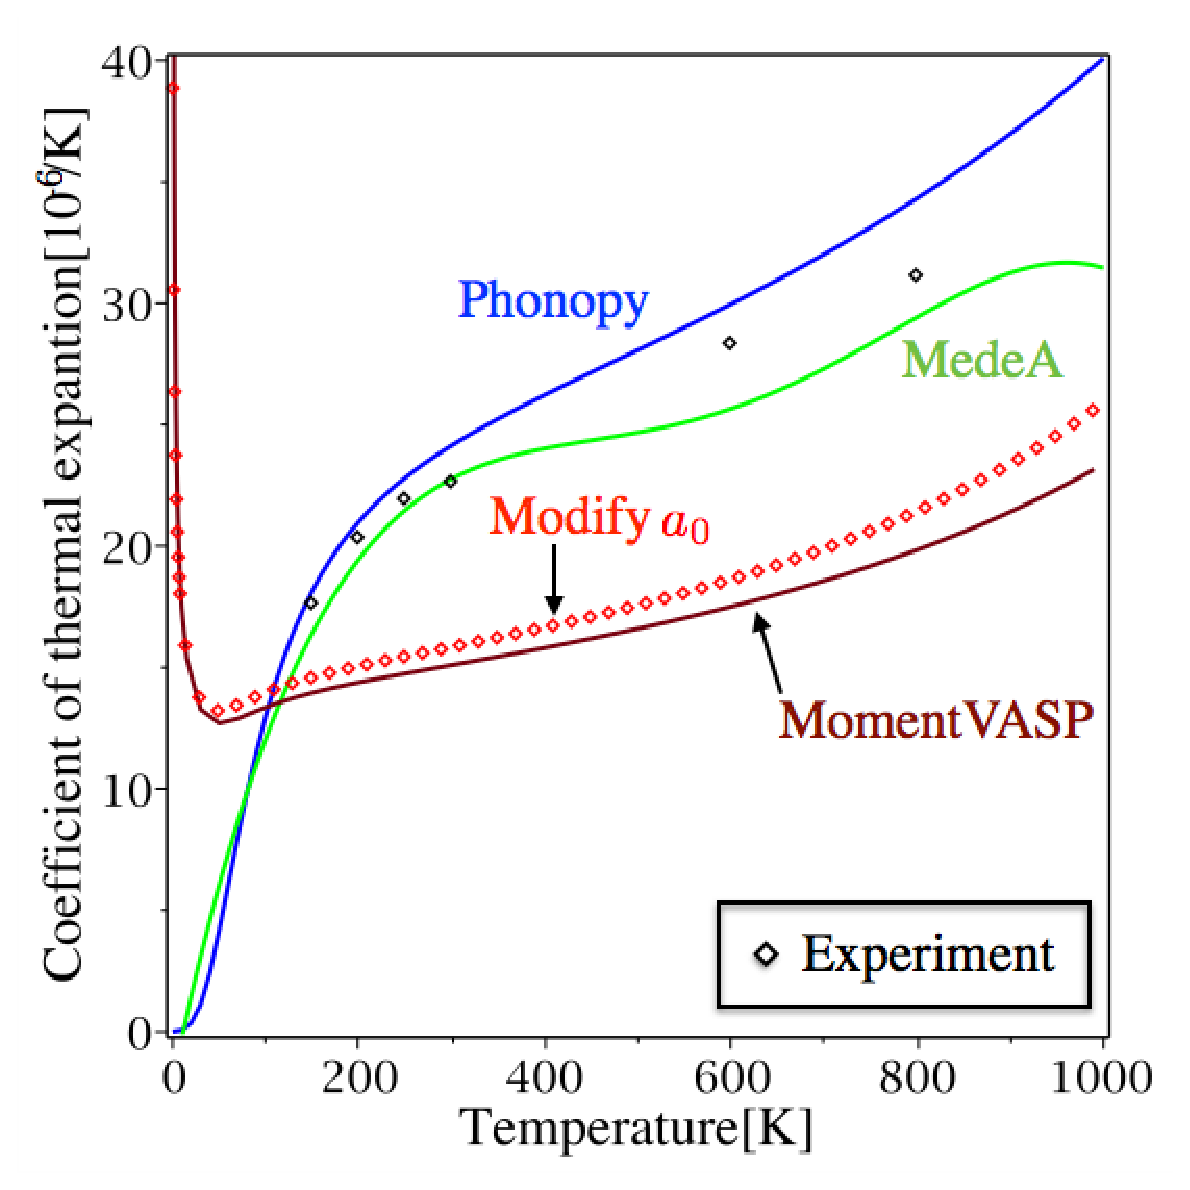
\includegraphics[keepaspectratio, scale=0.42]
  {../image_result/Al_TEcoeff_phonopy_label.eps}
  \subcaption{線膨張係数と温度の依存性.}\label{a0test2}
 \end{minipage}
 \hspace{10cm}
 \begin{minipage}[b]{0.5\linewidth}
  \centering
  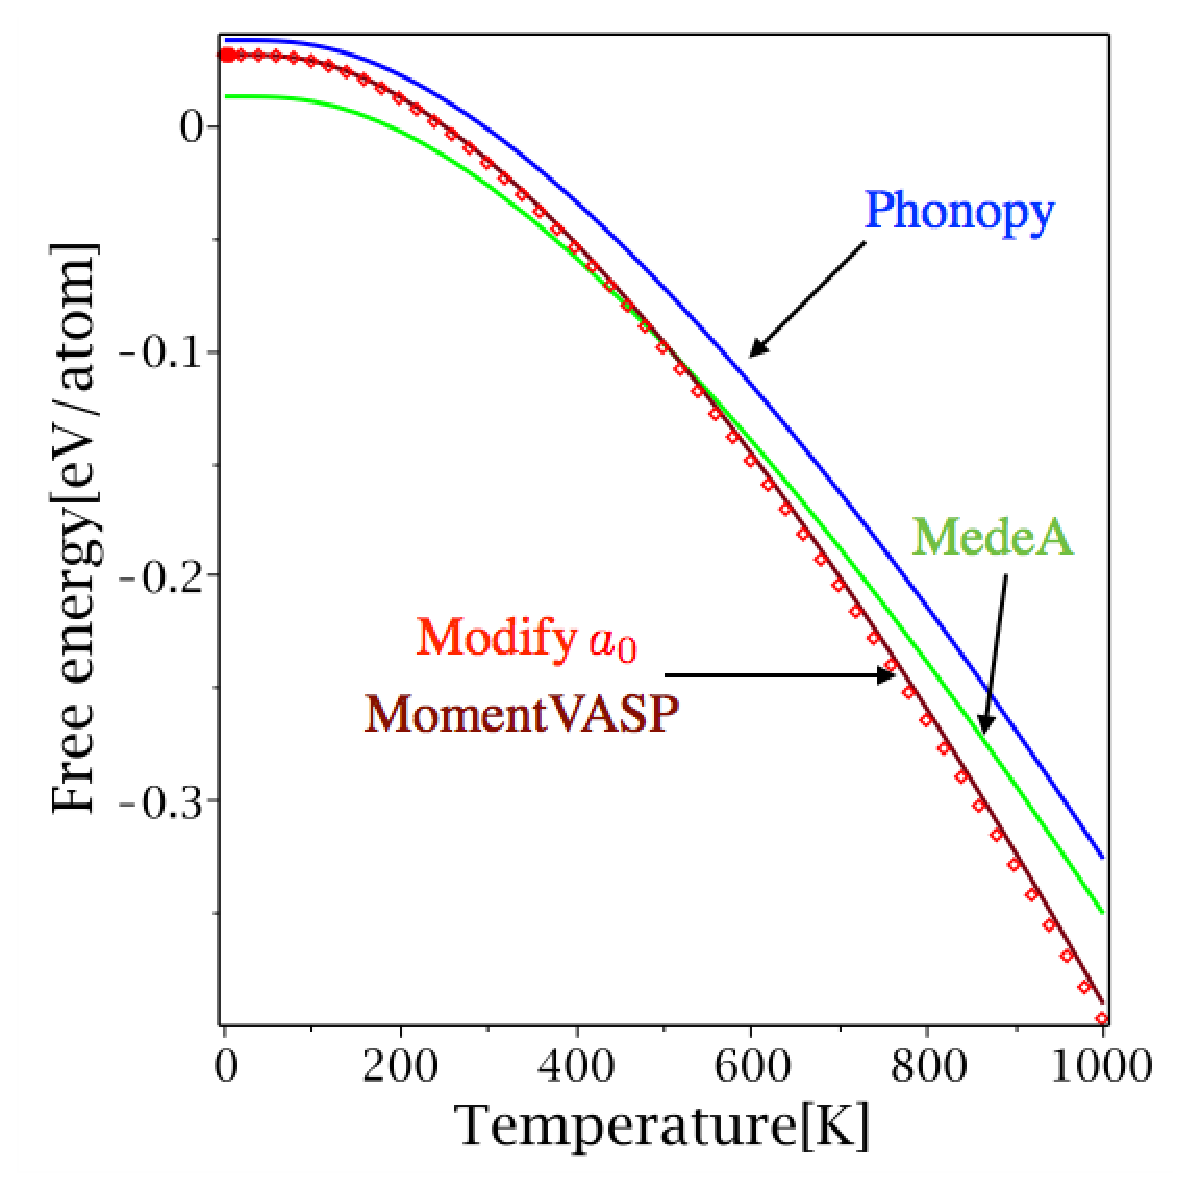
\includegraphics[keepaspectratio, scale=0.42]
  {../image_result/Al_free_phonopy_label.eps}
  \subcaption{$U_0$を含まない自由エネルギーの温度依存性.}\label{a0test3}
 \end{minipage}
 \begin{minipage}[b]{0.5\linewidth}
  \centering
  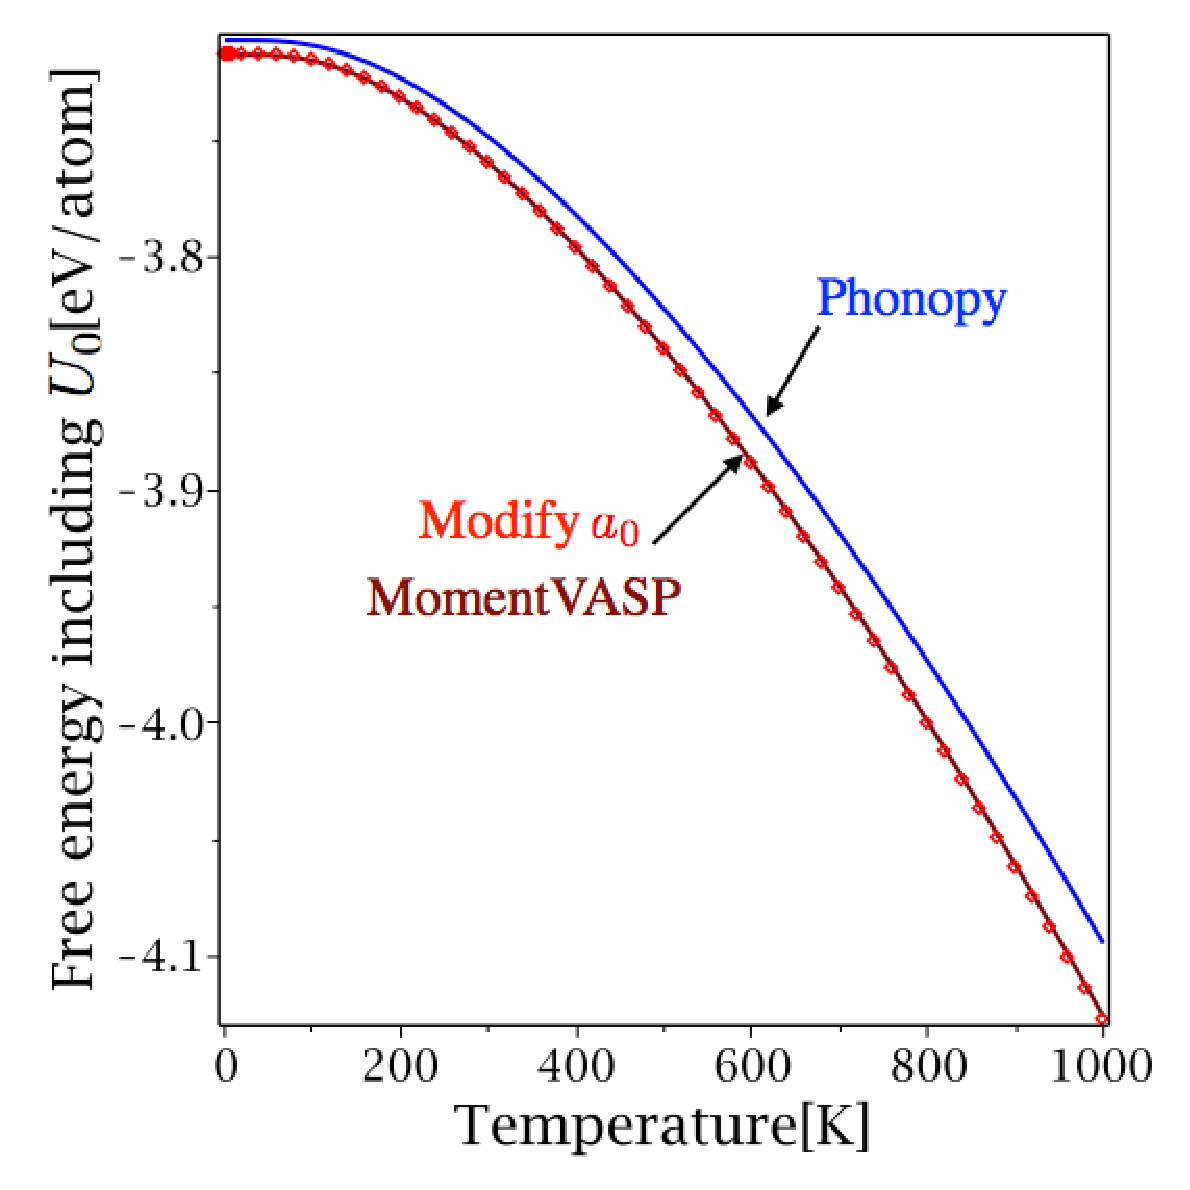
\includegraphics[keepaspectratio, scale=0.42]
  {../image_result/Al_free_u0_phonopy_label.eps}
  \subcaption{$U_0$を含んだ自由エネルギーの温度依存性.}\label{a0test4}
 \end{minipage}
 \caption{AlのMomentVASPの$a_0$をPhonopyの0Kでの最近接原子間距離に変えることによる計算結果の変化.}\label{fig:a0test}
\end{figure}

図中のラベルModify $a_0$がMomentVASPの$a_0$をPhonopyの0Kでの最近接原子間距離に変化させた計算結果である.
(\subref{a0test1})より,$a_0$をPhonopyと揃えたため0Kで同じ距離から熱膨張を開始しているが,その後の変化は元のMomentVaspとあまり変わらない結果となった.(\subref{a0test2})の線膨張係数で比較すると若干ではあるがPhonopyと実験値に近づいていることがわかる.
自由エネルギーの比較では(\subref{a0test3}),(\subref{a0test4})ともにModify $a_0$の値はPhonopyから遠ざかる方に変化している.
また,1000Kでの最近接原子間距離の差は強引ではあるが小さくなっているにも関わらず,自由エネルギーの値の差は小さくならなかった.
よって,0Kの最近節原子間距離をPhonopyと揃えるという試みは熱膨張係数のみ若干であるが改善されるという結果となった.

%考察
\chapter{総括}
本研究では,経験的ペアポテンシャルをでの計算を前提としているMoment法にVASPによる第一原理計算の結果の導入を試みた.
計算は対称性に優れており等方的な格子を持つfcc構造金属であるCu, Ag, Au, Alを対象とした.
Moment法の熱膨張の計算原理は線形結合を前提としている.従来のペアポテンシャルの計算では
原子をfcc構造で配置させそれぞれの原子に対して,x方向の2次,4次微分の総和をとることで線形結合に
対応していた.
それに対してVASPでの導入ではそれぞれの元素のユニットセルを格子の長さを変化させ第一原理計算を行い,結果からフィッティングにより関数を作る.
フィッティングにより得られたポテンシャル関数は3次元での計算結果であり,線形結合の熱膨張に対応させなければいけない.
そこで今回はfcc構造は等方性に優れているという点から3で割ることによって線形結合への対応を試みた.
これにより得られた計算に必要なパラメータ$k$, $\gamma$を用いて熱膨張,自由エネルギーの計算をした.
計算の信頼性を確かめるために,従来のペアポテンシャルを利用したMoment法,MedeA,PhonopyによるPhonon-DOS法と比較をおこなった.

結果をまとめると以下のようになる.
\begin{itemize}
 \item VASPを導入したMoment法は従来のペアポテンシャルのMoment法よりも,全ての計算でMedeA, Phonopy, 実験値に近い値をだした.
 \item Auの熱膨張はMedea, PhonopyではPhonon状態密度に負の値が混じり上手く再現できなかった.しかし,Phononとは違うアプローチで計算をするVASPを導入したMoment法では実験に近い数値を出すことができた.
  \item Alにおける熱膨張は,Phonopy, MedeAではよく再現することができている.しかし,VASPを導入したMoment法では熱膨張が小さいという結果になった.
 \item 内部エネルギーと熱膨張を考慮に入れたPhonopyの自由エネルギーの結果と比較すると,Cu, Agは比較的一致を見せた,Au, Alにおいては熱膨張に差があることもあり異なるカーブを描いた.
\end{itemize}
以上の結果より,VASPを導入したMoment法はある程度信頼できるということがわかった.

今後の課題としては,

\begin{itemize}
 \item 今回はfcc構造の等方性に注目し線形結合に対応するためにポテンシャルを3で割るという手法を試みた.これに対して,もっと良い手法がないか検討する.
 \item 今回の計算にはポテンシャルをフィッティングする際に7次の項まで利用したが,拾えていない成分が残っているかもしれない.そのため,フィッティング精度を高めてさらに高次の項まで取り込んだ計算を行えば違う結果が得られる可能性がある.
  \item 等方的ではないhcp構造での実装はどうするのか,$a$軸,$c$軸方向のポテンシャルは作ることができるが,それらからどのように実装するか考える必要がある.また,それにより負の膨張率の再現することができるか検証が必要である.
  \item $y_0$を近似によって求めているがもっと良い近似法がないか検証する.
\end{itemize}
以上が挙げられる.



%総括
\chapter*{謝辞} 
本研究を行うにあたり,終始多大なるご指導,御鞭撻をいただいた西谷滋人教授に対し,深く御礼申し上げます.また,本研究の進行に伴い,
様々な助力,知識の供給を頂きました西谷研究室の同輩,先輩方に心から感謝の意を示します.本当にありがとうございました.%謝辞
%参考文献

\begin{thebibliography}{9}
\bibitem{phonon}K. Parlinski, Z. Q. Li, and Y. Kawazoe, Phys. Rev. Let., {\bf 78} (1997), 4063-4066.
\bibitem{kiyohara}清原資之, 「Ti結晶多形におけるPhonon第一原理計算」, 関西学院大学 理工学部 卒業論文,2013. 
\bibitem{jindo}Vu Van Hung, and K. Masuda-Jindo, J. Phys. Soc. Jpn., {\bf 69} (2000), 2067.
\bibitem{jindo2}Nguyen Tang, and Vu Van Hung, Phys. Stat. Sol., {\bf 149} (1988), 511.
\bibitem{kittel}宇野良清, 津屋昇, 新関駒二郎, 森田章, 山下次郎, キッテル固体物理学入門 第8版(2005) p.139.
\bibitem{phonopy}Atsushi Togo and Isao Tanaka, Scr. Mater., {\bf108} (2015),1-5.
%\bibitem{akahon}西谷滋人著,「固体物理の基礎」(森北出版,2006).
\end{thebibliography}

\end{document}
%終了